%&preformat-synopsis
\RequirePackage[l2tabu,orthodox]{nag} % Раскомментировав, можно в логе получать рекомендации относительно правильного использования пакетов и предупреждения об устаревших и нерекомендуемых пакетах

% Откомментируйте, чтобы отключить генерацию закладок в pdf
% \PassOptionsToPackage{bookmarks=false}{hyperref}
\documentclass[a5paper,10pt,twoside,openany,article]{memoir} %,draft

%%%%%%%%%%%%%%%%%%%%%%%%%%%%%%%%%%%%%%%%%%%%%%%%%%%%%%%%%%%%%%%%%%%%%%%%%%%%%%%%
%%%% Файл упрощённых настроек шаблона, общих для диссертации и автореферата %%%%
%%%%%%%%%%%%%%%%%%%%%%%%%%%%%%%%%%%%%%%%%%%%%%%%%%%%%%%%%%%%%%%%%%%%%%%%%%%%%%%%

%%% Режим черновика %%%
\makeatletter
\@ifundefined{c@draft}{
  \newcounter{draft}
  \setcounter{draft}{0}  % 0 --- чистовик (максимальное соблюдение ГОСТ)
                         % 1 --- черновик (отклонения от ГОСТ, но быстрая
                         %       сборка итоговых PDF)
}{}
\makeatother

%%% Пометки в тексте %%%
\makeatletter
\@ifundefined{c@showmarkup}{
  \newcounter{showmarkup}
  \setcounter{showmarkup}{0}  % 0 --- скрыть пометки
                              % 1 --- показывать пометки
}{}
\makeatother

%%% Использование в pdflatex шрифтов не по-умолчанию %%%
\makeatletter
\@ifundefined{c@usealtfont}{
  \newcounter{usealtfont}
  \setcounter{usealtfont}{1}    % 0 --- шрифты на базе Computer Modern
                                % 1 --- использовать пакет pscyr, при его
                                %       наличии
                                % 2 --- использовать пакет XCharter, при наличии
                                %       подходящей версии
}{}
\makeatother

%%% Использование в xelatex и lualatex семейств шрифтов %%%
\makeatletter
\@ifundefined{c@fontfamily}{
  \newcounter{fontfamily}
  \setcounter{fontfamily}{1}  % 0 --- CMU семейство. Используется как fallback;
                              % 1 --- Шрифты от MS (Times New Roman и компания)
                              % 2 --- Семейство Liberation
}{}
\makeatother

%%% Библиография %%%
\makeatletter
\@ifundefined{c@bibliosel}{
  \newcounter{bibliosel}
  \setcounter{bibliosel}{0}   % 0 --- встроенная реализация с загрузкой файла
                              %       через движок bibtex8;
                              % 1 --- реализация пакетом biblatex через движок
                              %       biber
}{}
\makeatother

%%% Вывод типов ссылок в библиографии %%%
\makeatletter
\@ifundefined{c@mediadisplay}{
  \newcounter{mediadisplay}
  \setcounter{mediadisplay}{1}   % 0 --- не делать ничего; надписи [Текст] и
                                 %       [Эл. ресурс] будут выводиться только в ссылках с
                                 %       заполненным полем `media`;
                                 % 1 --- автоматически добавлять надпись [Текст] к ссылкам с
                                 %       незаполненным полем `media`; таким образом, у всех
                                 %       источников будет указан тип, что соответствует
                                 %       требованиям ГОСТ
                                 % 2 --- автоматически удалять надписи [Текст], [Эл. Ресурс] и др.;
                                 %       не соответствует ГОСТ
                                 % 3 --- автоматически удалять надпись [Текст];
                                 %       не соответствует ГОСТ
                                 % 4 --- автоматически удалять надпись [Эл. Ресурс];
                                 %       не соответствует ГОСТ
}{}
\makeatother

%%% Предкомпиляция tikz рисунков для ускорения работы %%%
\makeatletter
\@ifundefined{c@imgprecompile}{
  \newcounter{imgprecompile}
  \setcounter{imgprecompile}{0}   % 0 --- без предкомпиляции;
                                  % 1 --- пользоваться предварительно
                                  %       скомпилированными pdf вместо генерации
                                  %       заново из tikz
}{}
\makeatother
          % общие настройки шаблона
\input{common/packages}       % Пакеты общие для диссертации и автореферата
\synopsistrue                 % Этот документ --- автореферат
\input{Synopsis/synpackages}  % Пакеты для автореферата
\usepackage{fr-longtable}    %ради \endlasthead

% Листинги с исходным кодом программ
\usepackage{fancyvrb}
\usepackage{listings}
\lccode`\~=0\relax %Без этого хака из-за особенностей пакета listings перестают работать конструкции с \MakeLowercase и т. п. в (xe|lua)latex

% Русская традиция начертания греческих букв
\usepackage{upgreek} % прямые греческие ради русской традиции

%%% Микротипографика
\ifnumequal{\value{draft}}{0}{% Только если у нас режим чистовика
    \usepackage[final, babel, shrink=45]{microtype}[2016/05/14] % улучшает представление букв и слов в строках, может помочь при наличии отдельно висящих слов
}{}

% Отметка о версии черновика на каждой странице
% Чтобы работало надо в своей локальной копии по инструкции
% https://www.ctan.org/pkg/gitinfo2 создать небходимые файлы в папке
% ./git/hooks
% If you’re familiar with tweaking git, you can probably work it out for
% yourself. If not, I suggest you follow these steps:
% 1. First, you need a git repository and working tree. For this example,
% let’s suppose that the root of the working tree is in ~/compsci
% 2. Copy the file post-xxx-sample.txt (which is in the same folder of
% your TEX distribution as this pdf) into the git hooks directory in your
% working copy. In our example case, you should end up with a file called
% ~/compsci/.git/hooks/post-checkout
% 3. If you’re using a unix-like system, don’t forget to make the file executable.
% Just how you do this is outside the scope of this manual, but one
% possible way is with commands such as this:
% chmod g+x post-checkout.
% 4. Test your setup with “git checkout master” (or another suitable branch
% name). This should generate copies of gitHeadInfo.gin in the directories
% you intended.
% 5. Now make two more copies of this file in the same directory (hooks),
% calling them post-commit and post-merge, and you’re done. As before,
% users of unix-like systems should ensure these files are marked as
% executable.
\ifnumequal{\value{draft}}{1}{% Черновик
   \IfFileExists{.git/gitHeadInfo.gin}{
      \usepackage[mark,pcount]{gitinfo2}
      \renewcommand{\gitMark}{rev.\gitAbbrevHash\quad\gitCommitterEmail\quad\gitAuthorIsoDate}
      \renewcommand{\gitMarkFormat}{\rmfamily\color{Gray}\small\bfseries}
   }{}
}{} % Пакеты для специфических пользовательских задач

% Новые переменные, которые могут использоваться во всём проекте
% ГОСТ 7.0.11-2011
% 9.2 Оформление текста автореферата диссертации
% 9.2.1 Общая характеристика работы включает в себя следующие основные структурные
% элементы:
% актуальность темы исследования;
\newcommand{\actualityTXT}{Актуальность темы исследования.}
% степень ее разработанности;
\newcommand{\progressTXT}{Степень разработанности темы исследования.}
% цели и задачи;
\newcommand{\aimTXT}{Целью}
\newcommand{\tasksTXT}{задачи}
% научную новизну;
\newcommand{\noveltyTXT}{Научная новизна.}
% теоретическую и практическую значимость работы;
%\newcommand{\influenceTXT}{Теоретическая и практическая значимость}
% или чаще используют просто
\newcommand{\thInfluenceTXT}{Теоретическая значимость.}
\newcommand{\prInfluenceTXT}{Практическая значимость.}
% методологию и методы исследования;
\newcommand{\methodsTXT}{Методология и методы исследования.}
% положения, выносимые на защиту;
\newcommand{\defpositionsTXT}{Основные положения, выносимые на~защиту:}
% степень достоверности и апробацию результатов.
\newcommand{\reliabilityTXT}{Достоверность}
\newcommand{\probationTXT}{Апробация работы.}

\newcommand{\contributionTXT}{Личный вклад.}
\newcommand{\publicationsTXT}{Публикации.}


%%% Заголовки библиографии:

% для автореферата:
\newcommand{\bibtitleauthor}{Публикации автора по теме диссертации}

% для стиля библиографии `\insertbiblioauthorgrouped`
\newcommand{\bibtitleauthorvak}{В изданиях из списка ВАК РФ}
\newcommand{\bibtitleauthorscopus}{В изданиях, входящих в международную базу цитирования Scopus}
\newcommand{\bibtitleauthorwos}{В изданиях, входящих в международную базу цитирования Web of Science}
\newcommand{\bibtitleauthorother}{В прочих изданиях}
\newcommand{\bibtitleauthorconf}{В сборниках трудов конференций}
\newcommand{\bibtitleauthorpatent}{Зарегистрированные патенты}
\newcommand{\bibtitleauthorprogram}{Зарегистрированные программы для ЭВМ}

% для стиля библиографии `\insertbiblioauthorimportant`:
\newcommand{\bibtitleauthorimportant}{Наиболее значимые \protect\MakeLowercase\bibtitleauthor}

% для списка литературы в диссертации и списка чужих работ в автореферате:
\newcommand{\bibtitlefull}{Список литературы} % (ГОСТ Р 7.0.11-2011, 4)
       % Новые переменные, которые могут использоваться во всём проекте
%%%%%%%%%%%%%%%%%%%%%%%%%%%%%%%%%%%%%%%%%%%%%%%%%%%%%%%
%%%% Файл упрощённых настроек шаблона автореферата %%%%
%%%%%%%%%%%%%%%%%%%%%%%%%%%%%%%%%%%%%%%%%%%%%%%%%%%%%%%

%%% Инициализирование переменных, не трогать!  %%%
\newcounter{showperssign}
\newcounter{showsecrsign}
\newcounter{showopplead}
%%%%%%%%%%%%%%%%%%%%%%%%%%%%%%%%%%%%%%%%%%%%%%%%%%%%%%%

%%% Список публикаций %%%
\makeatletter
\@ifundefined{c@usefootcite}{
  \newcounter{usefootcite}
  \setcounter{usefootcite}{0} % 0 --- два списка литературы;
                              % 1 --- список публикаций автора + цитирование
                              %       других работ в сносках
}{}
\makeatother

\makeatletter
\@ifundefined{c@bibgrouped}{
  \newcounter{bibgrouped}
  \setcounter{bibgrouped}{1}  % 0 --- единый список работ автора;
                              % 1 --- сгруппированные работы автора
}{}
\makeatother

%%% Область упрощённого управления оформлением %%%

%% Управление зазором между подрисуночной подписью и основным текстом %%
\setlength{\belowcaptionskip}{10pt plus 20pt minus 2pt}


%% Подпись таблиц %%

% смещение строк подписи после первой
\newcommand{\tabindent}{0cm}

% тип форматирования таблицы
% plain --- название и текст в одной строке
% split --- название и текст в разных строках
\newcommand{\tabformat}{plain}

%%% настройки форматирования таблицы `plain'

% выравнивание по центру подписи, состоящей из одной строки
% true  --- выравнивать
% false --- не выравнивать
\newcommand{\tabsinglecenter}{false}

% выравнивание подписи таблиц
% justified   --- выравнивать как обычный текст
% centering   --- выравнивать по центру
% centerlast  --- выравнивать по центру только последнюю строку
% centerfirst --- выравнивать по центру только первую строку
% raggedleft  --- выравнивать по правому краю
% raggedright --- выравнивать по левому краю
\newcommand{\tabjust}{justified}

% Разделитель записи «Таблица #» и названия таблицы
\newcommand{\tablabelsep}{~\cyrdash\ }

%%% настройки форматирования таблицы `split'

% положение названия таблицы
% \centering   --- выравнивать по центру
% \raggedleft  --- выравнивать по правому краю
% \raggedright --- выравнивать по левому краю
\newcommand{\splitformatlabel}{\raggedleft}

% положение текста подписи
% \centering   --- выравнивать по центру
% \raggedleft  --- выравнивать по правому краю
% \raggedright --- выравнивать по левому краю
\newcommand{\splitformattext}{\raggedright}

%% Подпись рисунков %%
%Разделитель записи «Рисунок #» и названия рисунка
\newcommand{\figlabelsep}{~\cyrdash\ }  % (ГОСТ 2.105, 4.3.1)
                                        % "--- здесь не работает

%Демонстрация подписи диссертанта на автореферате
\setcounter{showperssign}{1}  % 0 --- не показывать;
                              % 1 --- показывать
%Демонстрация подписи учёного секретаря на автореферате
\setcounter{showsecrsign}{1}  % 0 --- не показывать;
                              % 1 --- показывать
%Демонстрация информации об оппонентах и ведущей организации на автореферате
\setcounter{showopplead}{1}   % 0 --- не показывать;
                              % 1 --- показывать

%%% Цвета гиперссылок %%%
% Latex color definitions: http://latexcolor.com/
\definecolor{linkcolor}{rgb}{0.9,0,0}
\definecolor{citecolor}{rgb}{0,0.6,0}
\definecolor{urlcolor}{rgb}{0,0,1}
%\definecolor{linkcolor}{rgb}{0,0,0} %black
%\definecolor{citecolor}{rgb}{0,0,0} %black
%\definecolor{urlcolor}{rgb}{0,0,0} %black
        % Упрощённые настройки шаблона

%%% Основные сведения %%%
\newcommand{\thesisAuthorLastName}{Булатов}
\newcommand{\thesisAuthorOtherNames}{Виктор Геннадьевич}
\newcommand{\thesisAuthorInitials}{В.\,Г.}
\newcommand{\thesisAuthor}             % Диссертация, ФИО автора
{%
    \texorpdfstring{% \texorpdfstring takes two arguments and uses the first for (La)TeX and the second for pdf
        \thesisAuthorLastName~\thesisAuthorOtherNames% так будет отображаться на титульном листе или в тексте, где будет использоваться переменная
    }{%
        \thesisAuthorLastName, \thesisAuthorOtherNames% эта запись для свойств pdf-файла. В таком виде, если pdf будет обработан программами для сбора библиографических сведений, будет правильно представлена фамилия.
    }
}
\newcommand{\thesisAuthorShort}        % Диссертация, ФИО автора инициалами
{\thesisAuthorInitials~\thesisAuthorLastName}
%\newcommand{\thesisUdk}                % Диссертация, УДК
%{\fixme{xxx.xxx}}
\newcommand{\thesisTitle}              % Диссертация, название
{Методы оценивания качества  и многокритериальной оптимизации тематических моделей в библиотеке TopicNet}
\newcommand{\thesisSpecialtyNumber}    % Диссертация, специальность, номер
{05.13.18}
\newcommand{\thesisSpecialtyTitle}     % Диссертация, специальность, название (название взято с сайта ВАК для примера)
{Математическое моделирование, численные методы и комплексы программ}
\newcommand{\thesisDegree}             % Диссертация, ученая степень
{кандидата технических наук}
\newcommand{\thesisDegreeShort}        % Диссертация, ученая степень, краткая запись
{канд. техн. наук}
\newcommand{\thesisCity}               % Диссертация, город написания диссертации
{Москва}
\newcommand{\thesisYear}               % Диссертация, год написания диссертации
{\the\year}
\newcommand{\thesisOrganization}       % Диссертация, организация
{Федеральное государственное автономное образовательное учреждение высшего образования «Московский физико-технический институт (национальный исследовательский университет)»}
\newcommand{\thesisOrganizationShort}  % Диссертация, краткое название организации для доклада
{МФТИ (ГУ)}

\newcommand{\thesisInOrganization}     % Диссертация, организация в предложном падеже: Работа выполнена в ...
{\fixme{учреждении с~длинным длинным длинным длинным названием, в~котором
выполнялась данная диссертационная работа}}

%% \newcommand{\supervisorDead}{}           % Рисовать рамку вокруг фамилии
\newcommand{\supervisorFio}              % Научный руководитель, ФИО
{Воронцов Константин Вячеславович}
\newcommand{\supervisorRegalia}          % Научный руководитель, регалии
{доктор физико-математических наук}
\newcommand{\supervisorFioShort}         % Научный руководитель, ФИО
{К.\,В.~Воронцов}
\newcommand{\supervisorRegaliaShort}     % Научный руководитель, регалии
{д-р физ.-мат. наук}

%% \newcommand{\supervisorTwoDead}{}        % Рисовать рамку вокруг фамилии
%% \newcommand{\supervisorTwoFio}           % Второй научный руководитель, ФИО
%% {\fixme{Фамилия Имя Отчество}}
%% \newcommand{\supervisorTwoRegalia}       % Второй научный руководитель, регалии
%% {\fixme{уч. степень, уч. звание}}
%% \newcommand{\supervisorTwoFioShort}      % Второй научный руководитель, ФИО
%% {\fixme{И.\,О.~Фамилия}}
%% \newcommand{\supervisorTwoRegaliaShort}  % Второй научный руководитель, регалии
%% {\fixme{уч.~ст.,~уч.~зв.}}

\newcommand{\opponentOneFio}           % Оппонент 1, ФИО
{\fixme{Фамилия Имя Отчество}}
\newcommand{\opponentOneRegalia}       % Оппонент 1, регалии
{\fixme{доктор физико-математических наук, профессор}}
\newcommand{\opponentOneJobPlace}      % Оппонент 1, место работы
{\fixme{Не очень длинное название для места работы}}
\newcommand{\opponentOneJobPost}       % Оппонент 1, должность
{\fixme{старший научный сотрудник}}

\newcommand{\opponentTwoFio}           % Оппонент 2, ФИО
{\fixme{Фамилия Имя Отчество}}
\newcommand{\opponentTwoRegalia}       % Оппонент 2, регалии
{\fixme{кандидат физико-математических наук}}
\newcommand{\opponentTwoJobPlace}      % Оппонент 2, место работы
{\fixme{Основное место работы c длинным длинным длинным длинным названием}}
\newcommand{\opponentTwoJobPost}       % Оппонент 2, должность
{\fixme{старший научный сотрудник}}

%% \newcommand{\opponentThreeFio}         % Оппонент 3, ФИО
%% {\fixme{Фамилия Имя Отчество}}
%% \newcommand{\opponentThreeRegalia}     % Оппонент 3, регалии
%% {\fixme{кандидат физико-математических наук}}
%% \newcommand{\opponentThreeJobPlace}    % Оппонент 3, место работы
%% {\fixme{Основное место работы c длинным длинным длинным длинным названием}}
%% \newcommand{\opponentThreeJobPost}     % Оппонент 3, должность
%% {\fixme{старший научный сотрудник}}

\newcommand{\leadingOrganizationTitle} % Ведущая организация, дополнительные строки. Удалить, чтобы не отображать в автореферате
{\fixme{Федеральное государственное бюджетное образовательное учреждение высшего
профессионального образования с~длинным длинным длинным длинным названием}}

\newcommand{\defenseDate}              % Защита, дата
{\fixme{DD mmmmmmmm YYYY~г.~в~XX часов}}
\newcommand{\defenseCouncilNumber}     % Защита, номер диссертационного совета
{\fixme{Д\,123.456.78}}
\newcommand{\defenseCouncilTitle}      % Защита, учреждение диссертационного совета
{\fixme{Название учреждения}}
\newcommand{\defenseCouncilAddress}    % Защита, адрес учреждение диссертационного совета
{\fixme{Адрес}}
\newcommand{\defenseCouncilPhone}      % Телефон для справок
{\fixme{+7~(0000)~00-00-00}}

\newcommand{\defenseSecretaryFio}      % Секретарь диссертационного совета, ФИО
{\fixme{Фамилия Имя Отчество}}
\newcommand{\defenseSecretaryRegalia}  % Секретарь диссертационного совета, регалии
{\fixme{д-р~физ.-мат. наук}}            % Для сокращений есть ГОСТы, например: ГОСТ Р 7.0.12-2011 + http://base.garant.ru/179724/#block_30000

\newcommand{\synopsisLibrary}          % Автореферат, название библиотеки
{\fixme{Название библиотеки}}
\newcommand{\synopsisDate}             % Автореферат, дата рассылки
{\fixme{DD mmmmmmmm}\the\year~года}

% To avoid conflict with beamer class use \providecommand
\providecommand{\keywords}%            % Ключевые слова для метаданных PDF диссертации и автореферата
{}
           % Основные сведения
\input{common/fonts}          % Определение шрифтов (частичное)
%%% Шаблон %%%
\DeclareRobustCommand{\fixme}{\textcolor{red}}  % решаем проблему превращения
                                % названия цвета в результате \MakeUppercase,
                                % http://tex.stackexchange.com/a/187930,
                                % \DeclareRobustCommand protects \fixme
                                % from expanding inside \MakeUppercase
\AtBeginDocument{%
    \setlength{\parindent}{2.5em}                   % Абзацный отступ. Должен быть одинаковым по всему тексту и равен пяти знакам (ГОСТ Р 7.0.11-2011, 5.3.7).
}

%%% Таблицы %%%
\DeclareCaptionLabelSeparator{tabsep}{\tablabelsep} % нумерация таблиц
\DeclareCaptionFormat{split}{\splitformatlabel#1\par\splitformattext#3}

\captionsetup[table]{
        format=\tabformat,                % формат подписи (plain|hang)
        font=normal,                      % нормальные размер, цвет, стиль шрифта
        skip=.0pt,                        % отбивка под подписью
        parskip=.0pt,                     % отбивка между параграфами подписи
        position=above,                   % положение подписи
        justification=\tabjust,           % центровка
        indent=\tabindent,                % смещение строк после первой
        labelsep=tabsep,                  % разделитель
        singlelinecheck=\tabsinglecenter, % не выравнивать по центру, если умещается в одну строку
}

%%% Рисунки %%%
\DeclareCaptionLabelSeparator{figsep}{\figlabelsep} % нумерация рисунков

\captionsetup[figure]{
        format=plain,                     % формат подписи (plain|hang)
        font=normal,                      % нормальные размер, цвет, стиль шрифта
        skip=.0pt,                        % отбивка под подписью
        parskip=.0pt,                     % отбивка между параграфами подписи
        position=below,                   % положение подписи
        singlelinecheck=true,             % выравнивание по центру, если умещается в одну строку
        justification=centerlast,         % центровка
        labelsep=figsep,                  % разделитель
}

%%% Подписи подрисунков %%%
\DeclareCaptionSubType{figure}
\renewcommand\thesubfigure{\asbuk{subfigure}} % нумерация подрисунков
\ifsynopsis
\DeclareCaptionFont{norm}{\fontsize{10pt}{11pt}\selectfont}
\newcommand{\subfigureskip}{2.pt}
\else
\DeclareCaptionFont{norm}{\fontsize{14pt}{16pt}\selectfont}
\newcommand{\subfigureskip}{0.pt}
\fi

\captionsetup[subfloat]{
        labelfont=norm,                 % нормальный размер подписей подрисунков
        textfont=norm,                  % нормальный размер подписей подрисунков
        labelsep=space,                 % разделитель
        labelformat=brace,              % одна скобка справа от номера
        justification=centering,        % центровка
        singlelinecheck=true,           % выравнивание по центру, если умещается в одну строку
        skip=\subfigureskip,            % отбивка над подписью
        parskip=.0pt,                   % отбивка между параграфами подписи
        position=below,                 % положение подписи
}

%%% Настройки ссылок на рисунки, таблицы и др. %%%
% команды \cref...format отвечают за форматирование при помощи команды \cref
% команды \labelcref...format отвечают за форматирование при помощи команды \labelcref

\ifpresentation
\else
    \crefdefaultlabelformat{#2#1#3}

    % Уравнение
    \crefformat{equation}{(#2#1#3)} % одиночная ссылка с приставкой
    \labelcrefformat{equation}{(#2#1#3)} % одиночная ссылка без приставки
    \crefrangeformat{equation}{(#3#1#4) \cyrdash~(#5#2#6)} % диапазон ссылок с приставкой
    \labelcrefrangeformat{equation}{(#3#1#4) \cyrdash~(#5#2#6)} % диапазон ссылок без приставки
    \crefmultiformat{equation}{(#2#1#3)}{ и~(#2#1#3)}{, (#2#1#3)}{ и~(#2#1#3)} % перечисление ссылок с приставкой
    \labelcrefmultiformat{equation}{(#2#1#3)}{ и~(#2#1#3)}{, (#2#1#3)}{ и~(#2#1#3)} % перечисление без приставки

    % Подуравнение
    \crefformat{subequation}{(#2#1#3)} % одиночная ссылка с приставкой
    \labelcrefformat{subequation}{(#2#1#3)} % одиночная ссылка без приставки
    \crefrangeformat{subequation}{(#3#1#4) \cyrdash~(#5#2#6)} % диапазон ссылок с приставкой
    \labelcrefrangeformat{subequation}{(#3#1#4) \cyrdash~(#5#2#6)} % диапазон ссылок без приставки
    \crefmultiformat{subequation}{(#2#1#3)}{ и~(#2#1#3)}{, (#2#1#3)}{ и~(#2#1#3)} % перечисление ссылок с приставкой
    \labelcrefmultiformat{subequation}{(#2#1#3)}{ и~(#2#1#3)}{, (#2#1#3)}{ и~(#2#1#3)} % перечисление без приставки

    % Глава
    \crefformat{chapter}{#2#1#3} % одиночная ссылка с приставкой
    \labelcrefformat{chapter}{#2#1#3} % одиночная ссылка без приставки
    \crefrangeformat{chapter}{#3#1#4 \cyrdash~#5#2#6} % диапазон ссылок с приставкой
    \labelcrefrangeformat{chapter}{#3#1#4 \cyrdash~#5#2#6} % диапазон ссылок без приставки
    \crefmultiformat{chapter}{#2#1#3}{ и~#2#1#3}{, #2#1#3}{ и~#2#1#3} % перечисление ссылок с приставкой
    \labelcrefmultiformat{chapter}{#2#1#3}{ и~#2#1#3}{, #2#1#3}{ и~#2#1#3} % перечисление без приставки

    % Параграф
    \crefformat{section}{#2#1#3} % одиночная ссылка с приставкой
    \labelcrefformat{section}{#2#1#3} % одиночная ссылка без приставки
    \crefrangeformat{section}{#3#1#4 \cyrdash~#5#2#6} % диапазон ссылок с приставкой
    \labelcrefrangeformat{section}{#3#1#4 \cyrdash~#5#2#6} % диапазон ссылок без приставки
    \crefmultiformat{section}{#2#1#3}{ и~#2#1#3}{, #2#1#3}{ и~#2#1#3} % перечисление ссылок с приставкой
    \labelcrefmultiformat{section}{#2#1#3}{ и~#2#1#3}{, #2#1#3}{ и~#2#1#3} % перечисление без приставки

    % Приложение
    \crefformat{appendix}{#2#1#3} % одиночная ссылка с приставкой
    \labelcrefformat{appendix}{#2#1#3} % одиночная ссылка без приставки
    \crefrangeformat{appendix}{#3#1#4 \cyrdash~#5#2#6} % диапазон ссылок с приставкой
    \labelcrefrangeformat{appendix}{#3#1#4 \cyrdash~#5#2#6} % диапазон ссылок без приставки
    \crefmultiformat{appendix}{#2#1#3}{ и~#2#1#3}{, #2#1#3}{ и~#2#1#3} % перечисление ссылок с приставкой
    \labelcrefmultiformat{appendix}{#2#1#3}{ и~#2#1#3}{, #2#1#3}{ и~#2#1#3} % перечисление без приставки

    % Рисунок
    \crefformat{figure}{#2#1#3} % одиночная ссылка с приставкой
    \labelcrefformat{figure}{#2#1#3} % одиночная ссылка без приставки
    \crefrangeformat{figure}{#3#1#4 \cyrdash~#5#2#6} % диапазон ссылок с приставкой
    \labelcrefrangeformat{figure}{#3#1#4 \cyrdash~#5#2#6} % диапазон ссылок без приставки
    \crefmultiformat{figure}{#2#1#3}{ и~#2#1#3}{, #2#1#3}{ и~#2#1#3} % перечисление ссылок с приставкой
    \labelcrefmultiformat{figure}{#2#1#3}{ и~#2#1#3}{, #2#1#3}{ и~#2#1#3} % перечисление без приставки

    % Таблица
    \crefformat{table}{#2#1#3} % одиночная ссылка с приставкой
    \labelcrefformat{table}{#2#1#3} % одиночная ссылка без приставки
    \crefrangeformat{table}{#3#1#4 \cyrdash~#5#2#6} % диапазон ссылок с приставкой
    \labelcrefrangeformat{table}{#3#1#4 \cyrdash~#5#2#6} % диапазон ссылок без приставки
    \crefmultiformat{table}{#2#1#3}{ и~#2#1#3}{, #2#1#3}{ и~#2#1#3} % перечисление ссылок с приставкой
    \labelcrefmultiformat{table}{#2#1#3}{ и~#2#1#3}{, #2#1#3}{ и~#2#1#3} % перечисление без приставки

    % Листинг
    \crefformat{lstlisting}{#2#1#3} % одиночная ссылка с приставкой
    \labelcrefformat{lstlisting}{#2#1#3} % одиночная ссылка без приставки
    \crefrangeformat{lstlisting}{#3#1#4 \cyrdash~#5#2#6} % диапазон ссылок с приставкой
    \labelcrefrangeformat{lstlisting}{#3#1#4 \cyrdash~#5#2#6} % диапазон ссылок без приставки
    \crefmultiformat{lstlisting}{#2#1#3}{ и~#2#1#3}{, #2#1#3}{ и~#2#1#3} % перечисление ссылок с приставкой
    \labelcrefmultiformat{lstlisting}{#2#1#3}{ и~#2#1#3}{, #2#1#3}{ и~#2#1#3} % перечисление без приставки

    % Листинг
    \crefformat{ListingEnv}{#2#1#3} % одиночная ссылка с приставкой
    \labelcrefformat{ListingEnv}{#2#1#3} % одиночная ссылка без приставки
    \crefrangeformat{ListingEnv}{#3#1#4 \cyrdash~#5#2#6} % диапазон ссылок с приставкой
    \labelcrefrangeformat{ListingEnv}{#3#1#4 \cyrdash~#5#2#6} % диапазон ссылок без приставки
    \crefmultiformat{ListingEnv}{#2#1#3}{ и~#2#1#3}{, #2#1#3}{ и~#2#1#3} % перечисление ссылок с приставкой
    \labelcrefmultiformat{ListingEnv}{#2#1#3}{ и~#2#1#3}{, #2#1#3}{ и~#2#1#3} % перечисление без приставки
\fi

%%% Настройки гиперссылок %%%
\ifluatex
    \hypersetup{
        unicode,                % Unicode encoded PDF strings
    }
\fi

\hypersetup{
    linktocpage=true,           % ссылки с номера страницы в оглавлении, списке таблиц и списке рисунков
%    linktoc=all,                % both the section and page part are links
%    pdfpagelabels=false,        % set PDF page labels (true|false)
    plainpages=false,           % Forces page anchors to be named by the Arabic form  of the page number, rather than the formatted form
    colorlinks,                 % ссылки отображаются раскрашенным текстом, а не раскрашенным прямоугольником, вокруг текста
    linkcolor={linkcolor},      % цвет ссылок типа ref, eqref и подобных
    citecolor={citecolor},      % цвет ссылок-цитат
    urlcolor={urlcolor},        % цвет гиперссылок
%    hidelinks,                  % Hide links (removing color and border)
    pdftitle={\thesisTitle},    % Заголовок
    pdfauthor={\thesisAuthor},  % Автор
    pdfsubject={\thesisSpecialtyNumber\ \thesisSpecialtyTitle},      % Тема
%    pdfcreator={Создатель},     % Создатель, Приложение
%    pdfproducer={Производитель},% Производитель, Производитель PDF
    pdfkeywords={\keywords},    % Ключевые слова
    pdflang={ru},
}
\ifnumequal{\value{draft}}{1}{% Черновик
    \hypersetup{
        draft,
    }
}{}

%%% Списки %%%
% Используем короткое тире (endash) для ненумерованных списков (ГОСТ 2.105-95, пункт 4.1.7, требует дефиса, но так лучше смотрится)
\renewcommand{\labelitemi}{\normalfont\bfseries{--}}

% Перечисление строчными буквами латинского алфавита (ГОСТ 2.105-95, 4.1.7)
%\renewcommand{\theenumi}{\alph{enumi}}
%\renewcommand{\labelenumi}{\theenumi)}

% Перечисление строчными буквами русского алфавита (ГОСТ 2.105-95, 4.1.7)
\makeatletter
\AddEnumerateCounter{\asbuk}{\russian@alph}{щ}      % Управляем списками/перечислениями через пакет enumitem, а он 'не знает' про asbuk, потому 'учим' его
\makeatother
%\renewcommand{\theenumi}{\asbuk{enumi}} %первый уровень нумерации
%\renewcommand{\labelenumi}{\theenumi)} %первый уровень нумерации
\renewcommand{\theenumii}{\asbuk{enumii}} %второй уровень нумерации
\renewcommand{\labelenumii}{\theenumii)} %второй уровень нумерации
\renewcommand{\theenumiii}{\arabic{enumiii}} %третий уровень нумерации
\renewcommand{\labelenumiii}{\theenumiii)} %третий уровень нумерации

\setlist{nosep,%                                    % Единый стиль для всех списков (пакет enumitem), без дополнительных интервалов.
    labelindent=\parindent,leftmargin=*%            % Каждый пункт, подпункт и перечисление записывают с абзацного отступа (ГОСТ 2.105-95, 4.1.8)
}

%%% Правильная нумерация приложений, рисунков и формул %%%
%% По ГОСТ 2.105, п. 4.3.8 Приложения обозначают заглавными буквами русского алфавита,
%% начиная с А, за исключением букв Ё, З, Й, О, Ч, Ь, Ы, Ъ.
%% Здесь также переделаны все нумерации русскими буквами.
\ifxetexorluatex
    \makeatletter
    \def\russian@Alph#1{\ifcase#1\or
       А\or Б\or В\or Г\or Д\or Е\or Ж\or
       И\or К\or Л\or М\or Н\or
       П\or Р\or С\or Т\or У\or Ф\or Х\or
       Ц\or Ш\or Щ\or Э\or Ю\or Я\else\xpg@ill@value{#1}{russian@Alph}\fi}
    \def\russian@alph#1{\ifcase#1\or
       а\or б\or в\or г\or д\or е\or ж\or
       и\or к\or л\or м\or н\or
       п\or р\or с\or т\or у\or ф\or х\or
       ц\or ш\or щ\or э\or ю\or я\else\xpg@ill@value{#1}{russian@alph}\fi}
    \def\cyr@Alph#1{\ifcase#1\or
        А\or Б\or В\or Г\or Д\or Е\or Ж\or
        И\or К\or Л\or М\or Н\or
        П\or Р\or С\or Т\or У\or Ф\or Х\or
        Ц\or Ш\or Щ\or Э\or Ю\or Я\else\xpg@ill@value{#1}{cyr@Alph}\fi}
    \def\cyr@alph#1{\ifcase#1\or
        а\or б\or в\or г\or д\or е\or ж\or
        и\or к\or л\or м\or н\or
        п\or р\or с\or т\or у\or ф\or х\or
        ц\or ш\or щ\or э\or ю\or я\else\xpg@ill@value{#1}{cyr@alph}\fi}
    \makeatother
\else
    \makeatletter
    \if@uni@ode
      \def\russian@Alph#1{\ifcase#1\or
        А\or Б\or В\or Г\or Д\or Е\or Ж\or
        И\or К\or Л\or М\or Н\or
        П\or Р\or С\or Т\or У\or Ф\or Х\or
        Ц\or Ш\or Щ\or Э\or Ю\or Я\else\@ctrerr\fi}
    \else
      \def\russian@Alph#1{\ifcase#1\or
        \CYRA\or\CYRB\or\CYRV\or\CYRG\or\CYRD\or\CYRE\or\CYRZH\or
        \CYRI\or\CYRK\or\CYRL\or\CYRM\or\CYRN\or
        \CYRP\or\CYRR\or\CYRS\or\CYRT\or\CYRU\or\CYRF\or\CYRH\or
        \CYRC\or\CYRSH\or\CYRSHCH\or\CYREREV\or\CYRYU\or
        \CYRYA\else\@ctrerr\fi}
    \fi
    \if@uni@ode
      \def\russian@alph#1{\ifcase#1\or
        а\or б\or в\or г\or д\or е\or ж\or
        и\or к\or л\or м\or н\or
        п\or р\or с\or т\or у\or ф\or х\or
        ц\or ш\or щ\or э\or ю\or я\else\@ctrerr\fi}
    \else
      \def\russian@alph#1{\ifcase#1\or
        \cyra\or\cyrb\or\cyrv\or\cyrg\or\cyrd\or\cyre\or\cyrzh\or
        \cyri\or\cyrk\or\cyrl\or\cyrm\or\cyrn\or
        \cyrp\or\cyrr\or\cyrs\or\cyrt\or\cyru\or\cyrf\or\cyrh\or
        \cyrc\or\cyrsh\or\cyrshch\or\cyrerev\or\cyryu\or
        \cyrya\else\@ctrerr\fi}
    \fi
    \makeatother
\fi


%%http://www.linux.org.ru/forum/general/6993203#comment-6994589 (используется totcount)
\makeatletter
\def\formtotal#1#2#3#4#5{%
    \newcount\@c
    \@c\totvalue{#1}\relax
    \newcount\@last
    \newcount\@pnul
    \@last\@c\relax
    \divide\@last 10
    \@pnul\@last\relax
    \divide\@pnul 10
    \multiply\@pnul-10
    \advance\@pnul\@last
    \multiply\@last-10
    \advance\@last\@c
    #2%
    \ifnum\@pnul=1#5\else%
    \ifcase\@last#5\or#3\or#4\or#4\or#4\else#5\fi
    \fi
}
\makeatother

\newcommand{\formbytotal}[5]{\total{#1}~\formtotal{#1}{#2}{#3}{#4}{#5}}

%%% Команды рецензирования %%%
\ifboolexpr{ (test {\ifnumequal{\value{draft}}{1}}) or (test {\ifnumequal{\value{showmarkup}}{1}})}{
        \newrobustcmd{\todo}[1]{\textcolor{red}{#1}}
        \newrobustcmd{\note}[2][]{\ifstrempty{#1}{#2}{\textcolor{#1}{#2}}}
        \newenvironment{commentbox}[1][]%
        {\ifstrempty{#1}{}{\color{#1}}}%
        {}
}{
        \newrobustcmd{\todo}[1]{}
        \newrobustcmd{\note}[2][]{}
        \excludecomment{commentbox}
}


         % Стили общие для диссертации и автореферата
\input{Synopsis/synstyles}    % Стили для автореферата
% для вертикального центрирования ячеек в tabulary
\def\zz{\ifx\[$\else\aftergroup\zzz\fi}
%$ \] % <-- чиним подсветку синтаксиса в некоторых редакторах
\def\zzz{\setbox0\lastbox
\dimen0\dimexpr\extrarowheight + \ht0-\dp0\relax
\setbox0\hbox{\raise-.5\dimen0\box0}%
\ht0=\dimexpr\ht0+\extrarowheight\relax
\dp0=\dimexpr\dp0+\extrarowheight\relax
\box0
}

\lstdefinelanguage{Renhanced}%
{keywords={abbreviate,abline,abs,acos,acosh,action,add1,add,%
        aggregate,alias,Alias,alist,all,anova,any,aov,aperm,append,apply,%
        approx,approxfun,apropos,Arg,args,array,arrows,as,asin,asinh,%
        atan,atan2,atanh,attach,attr,attributes,autoload,autoloader,ave,%
        axis,backsolve,barplot,basename,besselI,besselJ,besselK,besselY,%
        beta,binomial,body,box,boxplot,break,browser,bug,builtins,bxp,by,%
        c,C,call,Call,case,cat,category,cbind,ceiling,character,char,%
        charmatch,check,chol,chol2inv,choose,chull,class,close,cm,codes,%
        coef,coefficients,co,col,colnames,colors,colours,commandArgs,%
        comment,complete,complex,conflicts,Conj,contents,contour,%
        contrasts,contr,control,helmert,contrib,convolve,cooks,coords,%
        distance,coplot,cor,cos,cosh,count,fields,cov,covratio,wt,CRAN,%
        create,crossprod,cummax,cummin,cumprod,cumsum,curve,cut,cycle,D,%
        data,dataentry,date,dbeta,dbinom,dcauchy,dchisq,de,debug,%
        debugger,Defunct,default,delay,delete,deltat,demo,de,density,%
        deparse,dependencies,Deprecated,deriv,description,detach,%
        dev2bitmap,dev,cur,deviance,off,prev,,dexp,df,dfbetas,dffits,%
        dgamma,dgeom,dget,dhyper,diag,diff,digamma,dim,dimnames,dir,%
        dirname,dlnorm,dlogis,dnbinom,dnchisq,dnorm,do,dotplot,double,%
        download,dpois,dput,drop,drop1,dsignrank,dt,dummy,dump,dunif,%
        duplicated,dweibull,dwilcox,dyn,edit,eff,effects,eigen,else,%
        emacs,end,environment,env,erase,eval,equal,evalq,example,exists,%
        exit,exp,expand,expression,External,extract,extractAIC,factor,%
        fail,family,fft,file,filled,find,fitted,fivenum,fix,floor,for,%
        For,formals,format,formatC,formula,Fortran,forwardsolve,frame,%
        frequency,ftable,ftable2table,function,gamma,Gamma,gammaCody,%
        gaussian,gc,gcinfo,gctorture,get,getenv,geterrmessage,getOption,%
        getwd,gl,glm,globalenv,gnome,GNOME,graphics,gray,grep,grey,grid,%
        gsub,hasTsp,hat,heat,help,hist,home,hsv,httpclient,I,identify,if,%
        ifelse,Im,image,\%in\%,index,influence,measures,inherits,install,%
        installed,integer,interaction,interactive,Internal,intersect,%
        inverse,invisible,IQR,is,jitter,kappa,kronecker,labels,lapply,%
        layout,lbeta,lchoose,lcm,legend,length,levels,lgamma,library,%
        licence,license,lines,list,lm,load,local,locator,log,log10,log1p,%
        log2,logical,loglin,lower,lowess,ls,lsfit,lsf,ls,machine,Machine,%
        mad,mahalanobis,make,link,margin,match,Math,matlines,mat,matplot,%
        matpoints,matrix,max,mean,median,memory,menu,merge,methods,min,%
        missing,Mod,mode,model,response,mosaicplot,mtext,mvfft,na,nan,%
        names,omit,nargs,nchar,ncol,NCOL,new,next,NextMethod,nextn,%
        nlevels,nlm,noquote,NotYetImplemented,NotYetUsed,nrow,NROW,null,%
        numeric,\%o\%,objects,offset,old,on,Ops,optim,optimise,optimize,%
        options,or,order,ordered,outer,package,packages,page,pairlist,%
        pairs,palette,panel,par,parent,parse,paste,path,pbeta,pbinom,%
        pcauchy,pchisq,pentagamma,persp,pexp,pf,pgamma,pgeom,phyper,pico,%
        pictex,piechart,Platform,plnorm,plogis,plot,pmatch,pmax,pmin,%
        pnbinom,pnchisq,pnorm,points,poisson,poly,polygon,polyroot,pos,%
        postscript,power,ppoints,ppois,predict,preplot,pretty,Primitive,%
        print,prmatrix,proc,prod,profile,proj,prompt,prop,provide,%
        psignrank,ps,pt,ptukey,punif,pweibull,pwilcox,q,qbeta,qbinom,%
        qcauchy,qchisq,qexp,qf,qgamma,qgeom,qhyper,qlnorm,qlogis,qnbinom,%
        qnchisq,qnorm,qpois,qqline,qqnorm,qqplot,qr,Q,qty,qy,qsignrank,%
        qt,qtukey,quantile,quasi,quit,qunif,quote,qweibull,qwilcox,%
        rainbow,range,rank,rbeta,rbind,rbinom,rcauchy,rchisq,Re,read,csv,%
        csv2,fwf,readline,socket,real,Recall,rect,reformulate,regexpr,%
        relevel,remove,rep,repeat,replace,replications,report,require,%
        resid,residuals,restart,return,rev,rexp,rf,rgamma,rgb,rgeom,R,%
        rhyper,rle,rlnorm,rlogis,rm,rnbinom,RNGkind,rnorm,round,row,%
        rownames,rowsum,rpois,rsignrank,rstandard,rstudent,rt,rug,runif,%
        rweibull,rwilcox,sample,sapply,save,scale,scan,scan,screen,sd,se,%
        search,searchpaths,segments,seq,sequence,setdiff,setequal,set,%
        setwd,show,sign,signif,sin,single,sinh,sink,solve,sort,source,%
        spline,splinefun,split,sqrt,stars,start,stat,stem,step,stop,%
        storage,strstrheight,stripplot,strsplit,structure,strwidth,sub,%
        subset,substitute,substr,substring,sum,summary,sunflowerplot,svd,%
        sweep,switch,symbol,symbols,symnum,sys,status,system,t,table,%
        tabulate,tan,tanh,tapply,tempfile,terms,terrain,tetragamma,text,%
        time,title,topo,trace,traceback,transform,tri,trigamma,trunc,try,%
        ts,tsp,typeof,unclass,undebug,undoc,union,unique,uniroot,unix,%
        unlink,unlist,unname,untrace,update,upper,url,UseMethod,var,%
        variable,vector,Version,vi,warning,warnings,weighted,weights,%
        which,while,window,write,\%x\%,x11,X11,xedit,xemacs,xinch,xor,%
        xpdrows,xy,xyinch,yinch,zapsmall,zip},%
    otherkeywords={!,!=,~,$,*,\%,\&,\%/\%,\%*\%,\%\%,<-,<<-},%$
    alsoother={._$},%$
    sensitive,%
    morecomment=[l]\#,%
    morestring=[d]",%
    morestring=[d]'% 2001 Robert Denham
}%

%решаем проблему с кириллицей в комментариях (в pdflatex) https://tex.stackexchange.com/a/103712
\lstset{extendedchars=true,keepspaces=true,literate={Ö}{{\"O}}1
    {Ä}{{\"A}}1
    {Ü}{{\"U}}1
    {ß}{{\ss}}1
    {ü}{{\"u}}1
    {ä}{{\"a}}1
    {ö}{{\"o}}1
    {~}{{\textasciitilde}}1
    {а}{{\selectfont\char224}}1
    {б}{{\selectfont\char225}}1
    {в}{{\selectfont\char226}}1
    {г}{{\selectfont\char227}}1
    {д}{{\selectfont\char228}}1
    {е}{{\selectfont\char229}}1
    {ё}{{\"e}}1
    {ж}{{\selectfont\char230}}1
    {з}{{\selectfont\char231}}1
    {и}{{\selectfont\char232}}1
    {й}{{\selectfont\char233}}1
    {к}{{\selectfont\char234}}1
    {л}{{\selectfont\char235}}1
    {м}{{\selectfont\char236}}1
    {н}{{\selectfont\char237}}1
    {о}{{\selectfont\char238}}1
    {п}{{\selectfont\char239}}1
    {р}{{\selectfont\char240}}1
    {с}{{\selectfont\char241}}1
    {т}{{\selectfont\char242}}1
    {у}{{\selectfont\char243}}1
    {ф}{{\selectfont\char244}}1
    {х}{{\selectfont\char245}}1
    {ц}{{\selectfont\char246}}1
    {ч}{{\selectfont\char247}}1
    {ш}{{\selectfont\char248}}1
    {щ}{{\selectfont\char249}}1
    {ъ}{{\selectfont\char250}}1
    {ы}{{\selectfont\char251}}1
    {ь}{{\selectfont\char252}}1
    {э}{{\selectfont\char253}}1
    {ю}{{\selectfont\char254}}1
    {я}{{\selectfont\char255}}1
    {А}{{\selectfont\char192}}1
    {Б}{{\selectfont\char193}}1
    {В}{{\selectfont\char194}}1
    {Г}{{\selectfont\char195}}1
    {Д}{{\selectfont\char196}}1
    {Е}{{\selectfont\char197}}1
    {Ё}{{\"E}}1
    {Ж}{{\selectfont\char198}}1
    {З}{{\selectfont\char199}}1
    {И}{{\selectfont\char200}}1
    {Й}{{\selectfont\char201}}1
    {К}{{\selectfont\char202}}1
    {Л}{{\selectfont\char203}}1
    {М}{{\selectfont\char204}}1
    {Н}{{\selectfont\char205}}1
    {О}{{\selectfont\char206}}1
    {П}{{\selectfont\char207}}1
    {Р}{{\selectfont\char208}}1
    {С}{{\selectfont\char209}}1
    {Т}{{\selectfont\char210}}1
    {У}{{\selectfont\char211}}1
    {Ф}{{\selectfont\char212}}1
    {Х}{{\selectfont\char213}}1
    {Ц}{{\selectfont\char214}}1
    {Ч}{{\selectfont\char215}}1
    {Ш}{{\selectfont\char216}}1
    {Щ}{{\selectfont\char217}}1
    {Ъ}{{\selectfont\char218}}1
    {Ы}{{\selectfont\char219}}1
    {Ь}{{\selectfont\char220}}1
    {Э}{{\selectfont\char221}}1
    {Ю}{{\selectfont\char222}}1
    {Я}{{\selectfont\char223}}1
    {і}{{\selectfont\char105}}1
    {ї}{{\selectfont\char168}}1
    {є}{{\selectfont\char185}}1
    {ґ}{{\selectfont\char160}}1
    {І}{{\selectfont\char73}}1
    {Ї}{{\selectfont\char136}}1
    {Є}{{\selectfont\char153}}1
    {Ґ}{{\selectfont\char128}}1
}

% Ширина текста минус ширина надписи 999
\newlength{\twless}
\newlength{\lmarg}
\setlength{\lmarg}{\widthof{999}}   % ширина надписи 999
\setlength{\twless}{\textwidth-\lmarg}

\lstset{ %
%    language=R,                     %  Язык указать здесь, если во всех листингах преимущественно один язык, в результате часть настроек может пойти только для этого языка
    numbers=left,                   % where to put the line-numbers
    numberstyle=\fontsize{12pt}{14pt}\selectfont\color{Gray},  % the style that is used for the line-numbers
    firstnumber=1,                  % в этой и следующей строках задаётся поведение нумерации 5, 10, 15...
    stepnumber=5,                   % the step between two line-numbers. If it's 1, each line will be numbered
    numbersep=5pt,                  % how far the line-numbers are from the code
    backgroundcolor=\color{white},  % choose the background color. You must add \usepackage{color}
    showspaces=false,               % show spaces adding particular underscores
    showstringspaces=false,         % underline spaces within strings
    showtabs=false,                 % show tabs within strings adding particular underscores
    frame=leftline,                 % adds a frame of different types around the code
    rulecolor=\color{black},        % if not set, the frame-color may be changed on line-breaks within not-black text (e.g. commens (green here))
    tabsize=2,                      % sets default tabsize to 2 spaces
    captionpos=t,                   % sets the caption-position to top
    breaklines=true,                % sets automatic line breaking
    breakatwhitespace=false,        % sets if automatic breaks should only happen at whitespace
%    title=\lstname,                 % show the filename of files included with \lstinputlisting;
    % also try caption instead of title
    basicstyle=\fontsize{12pt}{14pt}\selectfont\ttfamily,% the size of the fonts that are used for the code
%    keywordstyle=\color{blue},      % keyword style
    commentstyle=\color{ForestGreen}\emph,% comment style
    stringstyle=\color{Mahogany},   % string literal style
    escapeinside={\%*}{*)},         % if you want to add a comment within your code
    morekeywords={*,...},           % if you want to add more keywords to the set
    inputencoding=utf8,             % кодировка кода
    xleftmargin={\lmarg},           % Чтобы весь код и полоска с номерами строк была смещена влево, так чтобы цифры не вылезали за пределы текста слева
}

%http://tex.stackexchange.com/questions/26872/smaller-frame-with-listings
% Окружение, чтобы листинг был компактнее обведен рамкой, если она задается, а не на всю ширину текста
\makeatletter
\newenvironment{SmallListing}[1][]
{\lstset{#1}\VerbatimEnvironment\begin{VerbatimOut}{VerbEnv.tmp}}
{\end{VerbatimOut}\settowidth\@tempdima{%
        \lstinputlisting{VerbEnv.tmp}}
    \minipage{\@tempdima}\lstinputlisting{VerbEnv.tmp}\endminipage}
\makeatother

\DefineVerbatimEnvironment% с шрифтом 12 пт
{Verb}{Verbatim}
{fontsize=\fontsize{12pt}{14pt}\selectfont}

\newfloat[chapter]{ListingEnv}{lol}{Листинг}

\renewcommand{\lstlistingname}{Листинг}

%Общие счётчики окружений листингов
%http://tex.stackexchange.com/questions/145546/how-to-make-figure-and-listing-share-their-counter
% Если смешивать плавающие и не плавающие окружения, то могут быть проблемы с нумерацией
\makeatletter
\AtBeginDocument{%
    \let\c@ListingEnv\c@lstlisting
    \let\theListingEnv\thelstlisting
    \let\ftype@lstlisting\ftype@ListingEnv % give the floats the same precedence
}
\makeatother

% значок С++ — используйте команду \cpp
\newcommand{\cpp}{%
    C\nolinebreak\hspace{-.05em}%
    \raisebox{.2ex}{+}\nolinebreak\hspace{-.10em}%
    \raisebox{.2ex}{+}%
}

%%%  Чересстрочное форматирование таблиц
%% http://tex.stackexchange.com/questions/278362/apply-italic-formatting-to-every-other-row
\newcounter{rowcnt}
\newcommand\altshape{\ifnumodd{\value{rowcnt}}{\color{red}}{\vspace*{-1ex}\itshape}}
% \AtBeginEnvironment{tabular}{\setcounter{rowcnt}{1}}
% \AtEndEnvironment{tabular}{\setcounter{rowcnt}{0}}

%%% Ради примера во второй главе
\let\originalepsilon\epsilon
\let\originalphi\phi
\let\originalkappa\kappa
\let\originalle\le
\let\originalleq\leq
\let\originalge\ge
\let\originalgeq\geq
\let\originalemptyset\emptyset
\let\originaltan\tan
\let\originalcot\cot
\let\originalcsc\csc

%%% Русская традиция начертания математических знаков
\renewcommand{\le}{\ensuremath{\leqslant}}
\renewcommand{\leq}{\ensuremath{\leqslant}}
\renewcommand{\ge}{\ensuremath{\geqslant}}
\renewcommand{\geq}{\ensuremath{\geqslant}}
\renewcommand{\emptyset}{\varnothing}

%%% Русская традиция начертания математических функций (на случай копирования из зарубежных источников)
\renewcommand{\tan}{\operatorname{tg}}
\renewcommand{\cot}{\operatorname{ctg}}
\renewcommand{\csc}{\operatorname{cosec}}

%%% Русская традиция начертания греческих букв (греческие буквы вертикальные, через пакет upgreek)
\renewcommand{\epsilon}{\ensuremath{\upvarepsilon}}   %  русская традиция записи
\renewcommand{\phi}{\ensuremath{\upvarphi}}
%\renewcommand{\kappa}{\ensuremath{\varkappa}}
\renewcommand{\alpha}{\upalpha}
\renewcommand{\beta}{\upbeta}
\renewcommand{\gamma}{\upgamma}
\renewcommand{\delta}{\updelta}
\renewcommand{\varepsilon}{\upvarepsilon}
\renewcommand{\zeta}{\upzeta}
\renewcommand{\eta}{\upeta}
\renewcommand{\theta}{\uptheta}
\renewcommand{\vartheta}{\upvartheta}
\renewcommand{\iota}{\upiota}
\renewcommand{\kappa}{\upkappa}
\renewcommand{\lambda}{\uplambda}
\renewcommand{\mu}{\upmu}
\renewcommand{\nu}{\upnu}
\renewcommand{\xi}{\upxi}
\renewcommand{\pi}{\uppi}
\renewcommand{\varpi}{\upvarpi}
\renewcommand{\rho}{\uprho}
%\renewcommand{\varrho}{\upvarrho}
\renewcommand{\sigma}{\upsigma}
%\renewcommand{\varsigma}{\upvarsigma}
\renewcommand{\tau}{\uptau}
\renewcommand{\upsilon}{\upupsilon}
\renewcommand{\varphi}{\upvarphi}
\renewcommand{\chi}{\upchi}
\renewcommand{\psi}{\uppsi}
\renewcommand{\omega}{\upomega}





% https://tex.stackexchange.com/questions/151984/double-vertical-bar-notation
\usepackage{mathtools}

\DeclarePairedDelimiterX{\infdivx}[2]{(}{)}{%
  #1\;\delimsize\|\;#2%
}
\newcommand{\infdiv}{\infdivx}
%\DeclarePairedDelimiter{\norm}{\lVert}{\rVert}
\newcommand{\norm}{\mathop{\mathsf{norm}}\limits}

% перенос формул в тексте
\newcommand*{\hm}[1]{#1\nobreak\discretionary {}%
{\hbox{$\mathsurround=0pt #1$}}{}}


\definecolor{my-red}{RGB}{176, 0, 0}
\definecolor{my-pink}{RGB}{253, 123, 124}

\newcommand\dscl[1]{\textbf{\textcolor{blue}{Оговорка: #1}}}

\newcommand{\bsym}{\boldsymbol}


\usepackage{algorithm} %[ruled]
\usepackage{algorithmicx}
\usepackage[noend]{algpseudocode} %[noend]
\renewcommand{\thealgorithm}{\arabic{algorithm}.}% Algorithm # is <chapter>.<algorithm>
\usepackage{fancybox}
\newsavebox{\algbox} % http://tex.stackexchange.com/questions/356427/add-equation-number-beside-algorithm/356458

\newcommand{\cond}{\mspace{2mu}{|}\mspace{2mu}}   % Стили для специфических пользовательских задач

%%% Библиография. Выбор движка для реализации %%%
\ifnumequal{\value{bibliosel}}{0}{%
    %%% Реализация библиографии встроенными средствами посредством движка bibtex8 %%%

%%% Пакеты %%%
\usepackage{cite}                                   % Красивые ссылки на литературу


%%% Стили %%%
% \bibliographystyle{BibTeX-Styles/gost71sv.bst}    % Оформляем библиографию по ГОСТ 7.1 (ГОСТ Р 7.0.11-2011, 5.6.7)
\bibliographystyle{BibTeX-Styles/utf8gost71s.bst}    % Оформляем библиографию по ГОСТ 7.1 (ГОСТ Р 7.0.11-2011, 5.6.7)
% буква s означает сортировать по алфавиту

\makeatletter
\renewcommand{\@biblabel}[1]{#1.}   % Заменяем библиографию с квадратных скобок на точку
\makeatother
%% Управление отступами между записями
%% требует etoolbox
%% http://tex.stackexchange.com/a/105642
%\patchcmd\thebibliography
% {\labelsep}
% {\labelsep\itemsep=5pt\parsep=0pt\relax}
% {}
% {\typeout{Couldn't patch the command}}

%%% Список литературы с красной строки (без висячего отступа) %%%
%\patchcmd{\thebibliography} %может потребовать включения пакета etoolbox
%  {\advance\leftmargin\labelsep}
%  {\leftmargin=0pt%
%   \setlength{\labelsep}{\widthof{\ }}% Управляет длиной отступа после точки
%   \itemindent=\parindent%
%   \addtolength{\itemindent}{\labelwidth}% Сдвигаем правее на величину номера с точкой
%   \advance\itemindent\labelsep%
%  }
%  {}{}

%%% Цитирование %%%
\renewcommand\citepunct{;\penalty\citepunctpenalty%
    \hskip.13emplus.1emminus.1em\relax}                % Разделение ; при перечислении ссылок (ГОСТ Р 7.0.5-2008)

\newcommand*{\autocite}[1]{}  % Чтобы примеры цитирования, рассчитанные на biblatex, не вызывали ошибок при компиляции в bibtex

%%% Создание команд для вывода списка литературы %%%
\newcommand*{\insertbibliofull}{
\bibliography{biblio/external,biblio/author}         % Подключаем BibTeX-базы % После запятых не должно быть лишних пробелов — он "думает", что это тоже имя пути
}

\newcommand*{\insertbiblioauthor}{
\bibliography{biblio/author}         % Подключаем BibTeX-базы % После запятых не должно быть лишних пробелов — он "думает", что это тоже имя пути
}

\newcommand*{\insertbiblioexternal}{
\bibliography{biblio/external}         % Подключаем BibTeX-базы
}


%% Счётчик использованных ссылок на литературу, обрабатывающий с учётом неоднократных ссылок
%% Требуется дважды компилировать, поскольку ему нужно считать актуальный внешний файл со списком литературы
\newtotcounter{citenum}
\def\oldcite{}
\let\oldcite=\bibcite
\def\bibcite{\stepcounter{citenum}\oldcite}
 % Встроенная реализация с загрузкой файла через движок bibtex8
}{
    %%% Реализация библиографии пакетами biblatex и biblatex-gost с использованием движка biber %%%

\usepackage{csquotes} % biblatex рекомендует его подключать. Пакет для оформления сложных блоков цитирования.
%%% Загрузка пакета с основными настройками %%%
\makeatletter
\ifnumequal{\value{draft}}{0}{% Чистовик
\usepackage[%
backend=biber,% движок
bibencoding=utf8,% кодировка bib файла
sorting=none,% настройка сортировки списка литературы
style=gost-numeric,% стиль цитирования и библиографии (по ГОСТ)
language=autobib,% получение языка из babel/polyglossia, default: autobib % если ставить autocite или auto, то цитаты в тексте с указанием страницы, получат указание страницы на языке оригинала
autolang=other,% многоязычная библиография
clearlang=true,% внутренний сброс поля language, если он совпадает с языком из babel/polyglossia
defernumbers=true,% нумерация проставляется после двух компиляций, зато позволяет выцеплять библиографию по ключевым словам и нумеровать не из большего списка
sortcites=true,% сортировать номера затекстовых ссылок при цитировании (если в квадратных скобках несколько ссылок, то отображаться будут отсортированно, а не абы как)
doi=false,% Показывать или нет ссылки на DOI
isbn=false,% Показывать или нет ISBN, ISSN, ISRN
]{biblatex}[2016/09/17]
\ltx@iffilelater{biblatex-gost.def}{2017/05/03}%
{\toggletrue{bbx:gostbibliography}%
\renewcommand*{\revsdnamepunct}{\addcomma}}{}
}{%Черновик
\usepackage[%
backend=biber,% движок
bibencoding=utf8,% кодировка bib файла
sorting=none,% настройка сортировки списка литературы
% defernumbers=true, % откомментируйте, если требуется правильная нумерация ссылок на литературу в режиме черновика. Замедляет сборку
]{biblatex}[2016/09/17]%
}
\makeatother

\providebool{blxmc} % biblatex version needs and has MakeCapital workaround
\boolfalse{blxmc} % setting our new boolean flag to default false
\ifxetexorluatex
\else
% Исправление случая неподдержки знака номера в pdflatex
    \DefineBibliographyStrings{russian}{number={\textnumero}}

% Исправление случая отсутствия прописных букв в некоторых случаях
% https://github.com/plk/biblatex/issues/960#issuecomment-596658282
    \ifdefmacro{\ExplSyntaxOn}{}{\usepackage{expl3}}
    \makeatletter
    \ltx@ifpackagelater{biblatex}{2020/02/23}{
    % Assuming this version of biblatex defines MakeCapital correctly
    }{
        \ltx@ifpackagelater{biblatex}{2019/12/01}{
            % Assuming this version of biblatex defines MakeCapital incorrectly
            \usepackage{expl3}[2020/02/25]
            \@ifpackagelater{expl3}{2020/02/25}{
                \booltrue{blxmc} % setting our new boolean flag to true
            }{}
        }{}
    }
    \makeatother
    \ifblxmc
        \typeout{Assuming this version of biblatex defines MakeCapital
        incorrectly}
        \usepackage{xparse}
        \makeatletter
        \ExplSyntaxOn
        \NewDocumentCommand \blx@maketext@lowercase {m}
          {
            \text_lowercase:n {#1}
          }

        \NewDocumentCommand \blx@maketext@uppercase {m}
          {
            \text_uppercase:n {#1}
          }

        \RenewDocumentCommand \MakeCapital {m}
          {
            \text_titlecase_first:n {#1}
          }
        \ExplSyntaxOff

        \protected\def\blx@biblcstring#1#2#3{%
          \blx@begunit
          \blx@hyphenreset
          \blx@bibstringsimple
          \lowercase{\edef\blx@tempa{#3}}%
          \ifcsundef{#2@\blx@tempa}
            {\blx@warn@nostring\blx@tempa
             \blx@endnounit}
            {#1{\blx@maketext@lowercase{\csuse{#2@\blx@tempa}}}%
             \blx@endunit}}

        \protected\def\blx@bibucstring#1#2#3{%
          \blx@begunit
          \blx@hyphenreset
          \blx@bibstringsimple
          \lowercase{\edef\blx@tempa{#3}}%
          \ifcsundef{#2@\blx@tempa}
            {\blx@warn@nostring\blx@tempa
             \blx@endnounit}
            {#1{\blx@maketext@uppercase{\csuse{#2@\blx@tempa}}}%
             \blx@endunit}}
        \makeatother
    \fi
\fi

\ifsynopsis
\ifnumgreater{\value{usefootcite}}{0}{
    \ExecuteBibliographyOptions{autocite=footnote}
    \newbibmacro*{cite:full}{%
        \printtext[bibhypertarget]{%
            \usedriver{%
                \DeclareNameAlias{sortname}{default}%
            }{%
                \thefield{entrytype}%
            }%
        }%
        \usebibmacro{shorthandintro}%
    }
    \DeclareCiteCommand{\smartcite}[\mkbibfootnote]{%
        \usebibmacro{prenote}%
    }{%
        \usebibmacro{citeindex}%
        \usebibmacro{cite:full}%
    }{%
        \multicitedelim%
    }{%
        \usebibmacro{postnote}%
    }
}{}
\fi

%%% Подключение файлов bib %%%
\addbibresource[label=bl-external]{biblio/external.bib}
\addbibresource[label=bl-author]{biblio/author.bib}
\addbibresource[label=bl-registered]{biblio/registered.bib}

%http://tex.stackexchange.com/a/141831/79756
%There is a way to automatically map the language field to the langid field. The following lines in the preamble should be enough to do that.
%This command will copy the language field into the langid field and will then delete the contents of the language field. The language field will only be deleted if it was successfully copied into the langid field.
\DeclareSourcemap{ %модификация bib файла перед тем, как им займётся biblatex
    \maps{
        \map{% перекидываем значения полей language в поля langid, которыми пользуется biblatex
            \step[fieldsource=language, fieldset=langid, origfieldval, final]
            \step[fieldset=language, null]
        }
        \map{% перекидываем значения полей numpages в поля pagetotal, которыми пользуется biblatex
            \step[fieldsource=numpages, fieldset=pagetotal, origfieldval, final]
            \step[fieldset=numpages, null]
        }
        \map{% перекидываем значения полей pagestotal в поля pagetotal, которыми пользуется biblatex
            \step[fieldsource=pagestotal, fieldset=pagetotal, origfieldval, final]
            \step[fieldset=pagestotal, null]
        }
        \map[overwrite]{% перекидываем значения полей shortjournal, если они есть, в поля journal, которыми пользуется biblatex
            \step[fieldsource=shortjournal, final]
            \step[fieldset=journal, origfieldval]
            \step[fieldset=shortjournal, null]
        }
        \map[overwrite]{% перекидываем значения полей shortbooktitle, если они есть, в поля booktitle, которыми пользуется biblatex
            \step[fieldsource=shortbooktitle, final]
            \step[fieldset=booktitle, origfieldval]
            \step[fieldset=shortbooktitle, null]
        }
        \map{% если в поле medium написано "Электронный ресурс", то устанавливаем поле media, которым пользуется biblatex, в значение eresource.
            \step[fieldsource=medium,
            match=\regexp{Электронный\s+ресурс},
            final]
            \step[fieldset=media, fieldvalue=eresource]
            \step[fieldset=medium, null]
        }
        \map[overwrite]{% стираем значения всех полей issn
            \step[fieldset=issn, null]
        }
        \map[overwrite]{% стираем значения всех полей abstract, поскольку ими не пользуемся, а там бывают "неприятные" латеху символы
            \step[fieldsource=abstract]
            \step[fieldset=abstract,null]
        }
        \map[overwrite]{ % переделка формата записи даты
            \step[fieldsource=urldate,
            match=\regexp{([0-9]{2})\.([0-9]{2})\.([0-9]{4})},
            replace={$3-$2-$1$4}, % $4 вставлен исключительно ради нормальной работы программ подсветки синтаксиса, которые некорректно обрабатывают $ в таких конструкциях
            final]
        }
        \map[overwrite]{ % стираем ключевые слова
            \step[fieldsource=keywords]
            \step[fieldset=keywords,null]
        }
        % реализация foreach различается для biblatex v3.12 и v3.13.
        % Для версии v3.13 эта конструкция заменяет последующие 7 структур map
        % \map[overwrite,foreach={authorvak,authorscopus,authorwos,authorconf,authorother,authorparent,authorprogram}]{ % записываем информацию о типе публикации в ключевые слова
        %     \step[fieldsource=$MAPLOOP,final=true]
        %     \step[fieldset=keywords,fieldvalue={,biblio$MAPLOOP},append=true]
        % }
        \map[overwrite]{ % записываем информацию о типе публикации в ключевые слова
            \step[fieldsource=authorvak,final=true]
            \step[fieldset=keywords,fieldvalue={,biblioauthorvak},append=true]
        }
        \map[overwrite]{ % записываем информацию о типе публикации в ключевые слова
            \step[fieldsource=authorscopus,final=true]
            \step[fieldset=keywords,fieldvalue={,biblioauthorscopus},append=true]
        }
        \map[overwrite]{ % записываем информацию о типе публикации в ключевые слова
            \step[fieldsource=authorwos,final=true]
            \step[fieldset=keywords,fieldvalue={,biblioauthorwos},append=true]
        }
        \map[overwrite]{ % записываем информацию о типе публикации в ключевые слова
            \step[fieldsource=authorconf,final=true]
            \step[fieldset=keywords,fieldvalue={,biblioauthorconf},append=true]
        }
        \map[overwrite]{ % записываем информацию о типе публикации в ключевые слова
            \step[fieldsource=authorother,final=true]
            \step[fieldset=keywords,fieldvalue={,biblioauthorother},append=true]
        }
        \map[overwrite]{ % записываем информацию о типе публикации в ключевые слова
            \step[fieldsource=authorpatent,final=true]
            \step[fieldset=keywords,fieldvalue={,biblioauthorpatent},append=true]
        }
        \map[overwrite]{ % записываем информацию о типе публикации в ключевые слова
            \step[fieldsource=authorprogram,final=true]
            \step[fieldset=keywords,fieldvalue={,biblioauthorprogram},append=true]
        }
        \map[overwrite]{ % добавляем ключевые слова, чтобы различать источники
            \perdatasource{biblio/external.bib}
            \step[fieldset=keywords, fieldvalue={,biblioexternal},append=true]
        }
        \map[overwrite]{ % добавляем ключевые слова, чтобы различать источники
            \perdatasource{biblio/author.bib}
            \step[fieldset=keywords, fieldvalue={,biblioauthor},append=true]
        }
        \map[overwrite]{ % добавляем ключевые слова, чтобы различать источники
            \perdatasource{biblio/registered.bib}
            \step[fieldset=keywords, fieldvalue={,biblioregistered},append=true]
        }
        \map[overwrite]{ % добавляем ключевые слова, чтобы различать источники
            \step[fieldset=keywords, fieldvalue={,bibliofull},append=true]
        }
%        \map[overwrite]{% стираем значения всех полей series
%            \step[fieldset=series, null]
%        }
        \map[overwrite]{% перекидываем значения полей howpublished в поля organization для типа online
            \step[typesource=online, typetarget=online, final]
            \step[fieldsource=howpublished, fieldset=organization, origfieldval]
            \step[fieldset=howpublished, null]
        }
    }
}

\ifnumequal{\value{mediadisplay}}{1}{
    \DeclareSourcemap{
        \maps{%
            \map{% использование media=text по умолчанию
                \step[fieldset=media, fieldvalue=text]
            }
        }
    }
}{}
\ifnumequal{\value{mediadisplay}}{2}{
    \DeclareSourcemap{
        \maps{%
            \map[overwrite]{% удаление всех записей media
                \step[fieldset=media, null]
            }
        }
    }
}{}
\ifnumequal{\value{mediadisplay}}{3}{
    \DeclareSourcemap{
        \maps{
            \map[overwrite]{% стираем значения всех полей media=text
                \step[fieldsource=media,match={text},final]
                \step[fieldset=media, null]
            }
        }
    }
}{}
\ifnumequal{\value{mediadisplay}}{4}{
    \DeclareSourcemap{
        \maps{
            \map[overwrite]{% стираем значения всех полей media=eresource
                \step[fieldsource=media,match={eresource},final]
                \step[fieldset=media, null]
            }
        }
    }
}{}

\ifsynopsis
\else
\DeclareSourcemap{ %модификация bib файла перед тем, как им займётся biblatex
    \maps{
        \map[overwrite]{% стираем значения всех полей addendum
            \perdatasource{biblio/author.bib}
            \step[fieldset=addendum, null] %чтобы избавиться от информации об объёме авторских статей, в отличие от автореферата
        }
    }
}
\fi

\ifpresentation
% удаляем лишние поля в списке литературы презентации
% их названия можно узнать в файле presentation.bbl
\DeclareSourcemap{
    \maps{
    \map[overwrite,foreach={%
        % {{{ Список лишних полей в презентации
        address,%
        chapter,%
        edition,%
        editor,%
        eid,%
        howpublished,%
        institution,%
        key,%
        month,%
        note,%
        number,%
        organization,%
        pages,%
        publisher,%
        school,%
        series,%
        type,%
        media,%
        url,%
        doi,%
        location,%
        volume,%
        % Список лишних полей в презентации }}}
    }]{
        \perdatasource{biblio/author.bib}
        \step[fieldset=$MAPLOOP,null]
    }
    }
}
\fi

\defbibfilter{vakscopuswos}{%
    keyword=biblioauthorvak or keyword=biblioauthorscopus or keyword=biblioauthorwos
}

\defbibfilter{scopuswos}{%
    keyword=biblioauthorscopus or keyword=biblioauthorwos
}

\defbibfilter{papersregistered}{%
    keyword=biblioauthor or keyword=biblioregistered
}

%%% Убираем неразрывные пробелы перед двоеточием и точкой с запятой %%%
%\makeatletter
%\ifnumequal{\value{draft}}{0}{% Чистовик
%    \renewcommand*{\addcolondelim}{%
%      \begingroup%
%      \def\abx@colon{%
%        \ifdim\lastkern>\z@\unkern\fi%
%        \abx@puncthook{:}\space}%
%      \addcolon%
%      \endgroup}
%
%    \renewcommand*{\addsemicolondelim}{%
%      \begingroup%
%      \def\abx@semicolon{%
%        \ifdim\lastkern>\z@\unkern\fi%
%        \abx@puncthook{;}\space}%
%      \addsemicolon%
%      \endgroup}
%}{}
%\makeatother

%%% Правка записей типа thesis, чтобы дважды не писался автор
%\ifnumequal{\value{draft}}{0}{% Чистовик
%\DeclareBibliographyDriver{thesis}{%
%  \usebibmacro{bibindex}%
%  \usebibmacro{begentry}%
%  \usebibmacro{heading}%
%  \newunit
%  \usebibmacro{author}%
%  \setunit*{\labelnamepunct}%
%  \usebibmacro{thesistitle}%
%  \setunit{\respdelim}%
%  %\printnames[last-first:full]{author}%Вот эту строчку нужно убрать, чтобы автор диссертации не дублировался
%  \newunit\newblock
%  \printlist[semicolondelim]{specdata}%
%  \newunit
%  \usebibmacro{institution+location+date}%
%  \newunit\newblock
%  \usebibmacro{chapter+pages}%
%  \newunit
%  \printfield{pagetotal}%
%  \newunit\newblock
%  \usebibmacro{doi+eprint+url+note}%
%  \newunit\newblock
%  \usebibmacro{addendum+pubstate}%
%  \setunit{\bibpagerefpunct}\newblock
%  \usebibmacro{pageref}%
%  \newunit\newblock
%  \usebibmacro{related:init}%
%  \usebibmacro{related}%
%  \usebibmacro{finentry}}
%}{}

%\newbibmacro{string+doi}[1]{% новая макрокоманда на простановку ссылки на doi
%    \iffieldundef{doi}{#1}{\href{http://dx.doi.org/\thefield{doi}}{#1}}}

%\ifnumequal{\value{draft}}{0}{% Чистовик
%\renewcommand*{\mkgostheading}[1]{\usebibmacro{string+doi}{#1}} % ссылка на doi с авторов. стоящих впереди записи
%\renewcommand*{\mkgostheading}[1]{#1} % только лишь убираем курсив с авторов
%}{}
%\DeclareFieldFormat{title}{\usebibmacro{string+doi}{#1}} % ссылка на doi с названия работы
%\DeclareFieldFormat{journaltitle}{\usebibmacro{string+doi}{#1}} % ссылка на doi с названия журнала
%%% Тире как разделитель в библиографии традиционной руской длины:
\renewcommand*{\newblockpunct}{\addperiod\addnbspace\cyrdash\space\bibsentence}
%%% Убрать тире из разделителей элементов в библиографии:
%\renewcommand*{\newblockpunct}{%
%    \addperiod\space\bibsentence}%block punct.,\bibsentence is for vol,etc.

%%% Возвращаем запись «Режим доступа» %%%
%\DefineBibliographyStrings{english}{%
%    urlfrom = {Mode of access}
%}
%\DeclareFieldFormat{url}{\bibstring{urlfrom}\addcolon\space\url{#1}}

%%% В списке литературы обозначение одной буквой диапазона страниц англоязычного источника %%%
\DefineBibliographyStrings{english}{%
    pages = {p\adddot} %заглавность буквы затем по месту определяется работой самого biblatex
}

%%% В ссылке на источник в основном тексте с указанием конкретной страницы обозначение одной большой буквой %%%
%\DefineBibliographyStrings{russian}{%
%    page = {C\adddot}
%}

%%% Исправление длины тире в диапазонах %%%
% \cyrdash --- тире «русской» длины, \textendash --- en-dash
\DefineBibliographyExtras{russian}{%
  \protected\def\bibrangedash{%
    \cyrdash\penalty\value{abbrvpenalty}}% almost unbreakable dash
  \protected\def\bibdaterangesep{\bibrangedash}%тире для дат
}
\DefineBibliographyExtras{english}{%
  \protected\def\bibrangedash{%
    \cyrdash\penalty\value{abbrvpenalty}}% almost unbreakable dash
  \protected\def\bibdaterangesep{\bibrangedash}%тире для дат
}

%Set higher penalty for breaking in number, dates and pages ranges
\setcounter{abbrvpenalty}{10000} % default is \hyphenpenalty which is 12

%Set higher penalty for breaking in names
\setcounter{highnamepenalty}{10000} % If you prefer the traditional BibTeX behavior (no linebreaks at highnamepenalty breakpoints), set it to ‘infinite’ (10 000 or higher).
\setcounter{lownamepenalty}{10000}

%%% Set low penalties for breaks at uppercase letters and lowercase letters
%\setcounter{biburllcpenalty}{500} %управляет разрывами ссылок после маленьких букв RTFM biburllcpenalty
%\setcounter{biburlucpenalty}{3000} %управляет разрывами ссылок после больших букв, RTFM biburlucpenalty

%%% Список литературы с красной строки (без висячего отступа) %%%
%\defbibenvironment{bibliography} % переопределяем окружение библиографии из gost-numeric.bbx пакета biblatex-gost
%  {\list
%     {\printtext[labelnumberwidth]{%
%       \printfield{prefixnumber}%
%       \printfield{labelnumber}}}
%     {%
%      \setlength{\labelwidth}{\labelnumberwidth}%
%      \setlength{\leftmargin}{0pt}% default is \labelwidth
%      \setlength{\labelsep}{\widthof{\ }}% Управляет длиной отступа после точки % default is \biblabelsep
%      \setlength{\itemsep}{\bibitemsep}% Управление дополнительным вертикальным разрывом между записями. \bibitemsep по умолчанию соответствует \itemsep списков в документе.
%      \setlength{\itemindent}{\bibhang}% Пользуемся тем, что \bibhang по умолчанию принимает значение \parindent (абзацного отступа), который переназначен в styles.tex
%      \addtolength{\itemindent}{\labelwidth}% Сдвигаем правее на величину номера с точкой
%      \addtolength{\itemindent}{\labelsep}% Сдвигаем ещё правее на отступ после точки
%      \setlength{\parsep}{\bibparsep}%
%     }%
%      \renewcommand*{\makelabel}[1]{\hss##1}%
%  }
%  {\endlist}
%  {\item}

%%% Макросы автоматического подсчёта количества авторских публикаций.
% Печатают невидимую (пустую) библиографию, считая количество источников.
% http://tex.stackexchange.com/a/66851/79756
%
\makeatletter
    \newtotcounter{citenum}
    \defbibenvironment{counter}
        {\setcounter{citenum}{0}\renewcommand{\blx@driver}[1]{}} % begin code: убирает весь выводимый текст
        {} % end code
        {\stepcounter{citenum}} % item code: cчитает "печатаемые в библиографию" источники

    \newtotcounter{citeauthorvak}
    \defbibenvironment{countauthorvak}
        {\setcounter{citeauthorvak}{0}\renewcommand{\blx@driver}[1]{}}
        {}
        {\stepcounter{citeauthorvak}}

    \newtotcounter{citeauthorscopus}
    \defbibenvironment{countauthorscopus}
        {\setcounter{citeauthorscopus}{0}\renewcommand{\blx@driver}[1]{}}
        {}
        {\stepcounter{citeauthorscopus}}

    \newtotcounter{citeauthorwos}
    \defbibenvironment{countauthorwos}
        {\setcounter{citeauthorwos}{0}\renewcommand{\blx@driver}[1]{}}
        {}
        {\stepcounter{citeauthorwos}}

    \newtotcounter{citeauthorother}
    \defbibenvironment{countauthorother}
        {\setcounter{citeauthorother}{0}\renewcommand{\blx@driver}[1]{}}
        {}
        {\stepcounter{citeauthorother}}

    \newtotcounter{citeauthorconf}
    \defbibenvironment{countauthorconf}
        {\setcounter{citeauthorconf}{0}\renewcommand{\blx@driver}[1]{}}
        {}
        {\stepcounter{citeauthorconf}}

    \newtotcounter{citeauthor}
    \defbibenvironment{countauthor}
        {\setcounter{citeauthor}{0}\renewcommand{\blx@driver}[1]{}}
        {}
        {\stepcounter{citeauthor}}

    \newtotcounter{citeauthorvakscopuswos}
    \defbibenvironment{countauthorvakscopuswos}
        {\setcounter{citeauthorvakscopuswos}{0}\renewcommand{\blx@driver}[1]{}}
        {}
        {\stepcounter{citeauthorvakscopuswos}}

    \newtotcounter{citeauthorscopuswos}
    \defbibenvironment{countauthorscopuswos}
        {\setcounter{citeauthorscopuswos}{0}\renewcommand{\blx@driver}[1]{}}
        {}
        {\stepcounter{citeauthorscopuswos}}

    \newtotcounter{citeregistered}
    \defbibenvironment{countregistered}
        {\setcounter{citeregistered}{0}\renewcommand{\blx@driver}[1]{}}
        {}
        {\stepcounter{citeregistered}}

    \newtotcounter{citeauthorpatent}
    \defbibenvironment{countauthorpatent}
        {\setcounter{citeauthorpatent}{0}\renewcommand{\blx@driver}[1]{}}
        {}
        {\stepcounter{citeauthorpatent}}

    \newtotcounter{citeauthorprogram}
    \defbibenvironment{countauthorprogram}
        {\setcounter{citeauthorprogram}{0}\renewcommand{\blx@driver}[1]{}}
        {}
        {\stepcounter{citeauthorprogram}}

    \newtotcounter{citeexternal}
    \defbibenvironment{countexternal}
        {\setcounter{citeexternal}{0}\renewcommand{\blx@driver}[1]{}}
        {}
        {\stepcounter{citeexternal}}
\makeatother

\defbibheading{nobibheading}{} % пустой заголовок, для подсчёта публикаций с помощью невидимой библиографии
\defbibheading{pubgroup}{\section*{#1}} % обычный стиль, заголовок-секция
\defbibheading{pubsubgroup}{\noindent\textbf{#1}} % для подразделов "по типу источника"

%%%Сортировка списка литературы Русский-Английский (предварительно удалить dissertation.bbl) (начало)
%%%Источник: https://github.com/odomanov/biblatex-gost/wiki/%D0%9A%D0%B0%D0%BA-%D1%81%D0%B4%D0%B5%D0%BB%D0%B0%D1%82%D1%8C,-%D1%87%D1%82%D0%BE%D0%B1%D1%8B-%D1%80%D1%83%D1%81%D1%81%D0%BA%D0%BE%D1%8F%D0%B7%D1%8B%D1%87%D0%BD%D1%8B%D0%B5-%D0%B8%D1%81%D1%82%D0%BE%D1%87%D0%BD%D0%B8%D0%BA%D0%B8-%D0%BF%D1%80%D0%B5%D0%B4%D1%88%D0%B5%D1%81%D1%82%D0%B2%D0%BE%D0%B2%D0%B0%D0%BB%D0%B8-%D0%BE%D1%81%D1%82%D0%B0%D0%BB%D1%8C%D0%BD%D1%8B%D0%BC
%\DeclareSourcemap{
%    \maps[datatype=bibtex]{
%        \map{
%            \step[fieldset=langid, fieldvalue={tempruorder}]
%        }
%        \map[overwrite]{
%            \step[fieldsource=langid, match=russian, final]
%            \step[fieldsource=presort,
%            match=\regexp{(.+)},
%            replace=\regexp{aa$1}]
%        }
%        \map{
%            \step[fieldsource=langid, match=russian, final]
%            \step[fieldset=presort, fieldvalue={az}]
%        }
%        \map[overwrite]{
%            \step[fieldsource=langid, notmatch=russian, final]
%            \step[fieldsource=presort,
%            match=\regexp{(.+)},
%            replace=\regexp{za$1}]
%        }
%        \map{
%            \step[fieldsource=langid, notmatch=russian, final]
%            \step[fieldset=presort, fieldvalue={zz}]
%        }
%        \map{
%            \step[fieldsource=langid, match={tempruorder}, final]
%            \step[fieldset=langid, null]
%        }
%    }
%}
%Сортировка списка литературы (конец)

%%% Создание команд для вывода списка литературы %%%
\newcommand*{\insertbibliofull}{
    \printbibliography[keyword=bibliofull,section=0,title=\bibtitlefull]
    \ifnumequal{\value{draft}}{0}{
      \printbibliography[heading=nobibheading,env=counter,keyword=bibliofull,section=0]
    }{}
}
\newcommand*{\insertbiblioauthor}{
    \printbibliography[heading=pubgroup, section=0, filter=papersregistered, title=\bibtitleauthor]
}
\newcommand*{\insertbiblioauthorimportant}{
    \printbibliography[heading=pubgroup, section=2, filter=papersregistered, title=\bibtitleauthorimportant]
}

% Вариант вывода печатных работ автора, с группировкой по типу источника.
% Порядок команд `\printbibliography` должен соответствовать порядку в файле common/characteristic.tex
\newcommand*{\insertbiblioauthorgrouped}{
    \section*{\bibtitleauthor}
    \ifsynopsis
    \printbibliography[heading=pubsubgroup, section=0, keyword=biblioauthorvak,    title=\bibtitleauthorvak,resetnumbers=true] % Работы автора из списка ВАК (сброс нумерации)
    \else
    \printbibliography[heading=pubsubgroup, section=0, keyword=biblioauthorvak,    title=\bibtitleauthorvak,resetnumbers=false] % Работы автора из списка ВАК (сквозная нумерация)
    \fi
    \printbibliography[heading=pubsubgroup, section=0, keyword=biblioauthorwos,    title=\bibtitleauthorwos,resetnumbers=false]% Работы автора, индексируемые Web of Science
    \printbibliography[heading=pubsubgroup, section=0, keyword=biblioauthorscopus, title=\bibtitleauthorscopus,resetnumbers=false]% Работы автора, индексируемые Scopus
    \printbibliography[heading=pubsubgroup, section=0, keyword=biblioauthorpatent, title=\bibtitleauthorpatent,resetnumbers=false]% Патенты
    \printbibliography[heading=pubsubgroup, section=0, keyword=biblioauthorprogram,title=\bibtitleauthorprogram,resetnumbers=false]% Программы для ЭВМ
    \printbibliography[heading=pubsubgroup, section=0, keyword=biblioauthorconf,   title=\bibtitleauthorconf,resetnumbers=false]% Тезисы конференций
    \printbibliography[heading=pubsubgroup, section=0, keyword=biblioauthorother,  title=\bibtitleauthorother,resetnumbers=false]% Прочие работы автора
}

\newcommand*{\insertbiblioexternal}{
    \printbibliography[heading=pubgroup,    section=0, keyword=biblioexternal,     title=\bibtitlefull]
}

\ExecuteBibliographyOptions{maxnames=99}

   % Реализация пакетом biblatex через движок biber
}

% Вывести информацию о выбранных опциях в лог сборки
\typeout{Selected options:}
\typeout{Draft mode: \arabic{draft}}
\typeout{Font: \arabic{fontfamily}}
\typeout{AltFont: \arabic{usealtfont}}
\typeout{Bibliography backend: \arabic{bibliosel}}
\typeout{Precompile images: \arabic{imgprecompile}}
% Вывести информацию о версиях используемых библиотек в лог сборки
\listfiles

\begin{document}

\thispagestyle{empty}

\noindent%
\begin{tabularx}{\textwidth}{@{}lXr@{}}%
    & & \large{На правах рукописи}\\
    \IfFileExists{images/empty.pdf}{\includegraphics[height=2.5cm]{empty}}{\rule[0pt]{0pt}{2.5cm}}  & &
    \ifnumequal{\value{showperssign}}{0}{%
        \rule[0pt]{0pt}{1.5cm}
    }{
        
\includegraphics[height=3.0cm]{personal-signature.png}
    }\\
\end{tabularx}

\vspace{0pt plus1fill} %число перед fill = кратность относительно некоторого расстояния fill, кусками которого заполнены пустые места
\begin{center}
\textbf {\large \thesisAuthor}
\end{center}

\vspace{0pt plus3fill} %число перед fill = кратность относительно некоторого расстояния fill, кусками которого заполнены пустые места
\begin{center}
\textbf {\Large %\MakeUppercase
\thesisTitle}

\vspace{0pt plus3fill} %число перед fill = кратность относительно некоторого расстояния fill, кусками которого заполнены пустые места
{\large Специальность \thesisSpecialtyNumber\ "---\par <<\thesisSpecialtyTitle>>}

\ifdefined\thesisSpecialtyTwoNumber
{\large Специальность \thesisSpecialtyTwoNumber\ "---\par <<\thesisSpecialtyTwoTitle>>}
\fi

\vspace{0pt plus1.5fill} %число перед fill = кратность относительно некоторого расстояния fill, кусками которого заполнены пустые места
\Large{Автореферат}\par
\large{диссертации на соискание учёной степени\par \thesisDegree}
\end{center}

\vspace{0pt plus4fill} %число перед fill = кратность относительно некоторого расстояния fill, кусками которого заполнены пустые места
{\centering\thesisCity~--- \thesisYear\par}

\newpage
% оборотная сторона обложки
\thispagestyle{empty}
{\centering
\noindent Работа прошла апробацию на {\thesisInOrganization}.
\par}

\vspace{0.008\paperheight}
\noindent%
\begin{tabularx}{\textwidth}{@{}lX@{}}
    \ifdefined\supervisorTwoFio
    Научные руководители:   & \supervisorRegalia\par
                              \ifdefined\supervisorDead
                              \framebox{\textbf{\supervisorFio}}
                              \else
                              \textbf{\supervisorFio}
                              \fi
                              \par
                              \vspace{0.013\paperheight}
                              \supervisorRegalia\par
                              \ifdefined\supervisorTwoDead
                              \framebox{\textbf{\supervisorTwoFio}}
                              \else
                              \textbf{\supervisorTwoFio}
                              \fi
                              \vspace{0.013\paperheight}\\
    \else
    Научный руководитель:   & \supervisorRegalia\par
                              \ifdefined\supervisorDead
                              \framebox{\textbf{\supervisorFio}}
                              \else
                              \textbf{\supervisorFio}
                              \fi
                              \vspace{0.013\paperheight}\\
    \fi
    \vspace{0.013\paperheight} 
    \ifdefined\leadingOrganizationTitle
    Ведущая организация:    &
    \ifnumequal{\value{showopplead}}{0}{\vspace{6\onelineskip plus1fill}}{%
        \leadingOrganizationTitle
    }%
    \fi
\end{tabularx}
\vspace{0.008\paperheight plus1fill}


\noindent Защита состоится \defenseDate~на~заседании диссертационного совета \defenseCouncilNumber~по адресу: \defenseCouncilAddress. \\
\\
\noindent С диссертацией можно ознакомиться  в библиотеке и на сайте Московского физико-технического института (национального исследовательского университета) \url{https://mipt.ru/education/post-graduate/ soiskateli-tekhnicheskie-nauki.php}.


\vspace{0.008\paperheight plus1fill}

\noindent Работа представлена <<15>> октября 2020~г. в~Аттестационную комиссию федерального государственного автономного образовательного учреждения высшего образования <<Московский физико-технический институт (национальный исследовательский университет)>> для рассмотрения советом по защите диссертаций на соискание ученой степени кандидата наук, доктора наук в соответствии с~п.3.1 ст.~4 Федерального закона <<О
науке и государственной научно-технической политике>>.

        % Титульный лист
%\mainmatter                   % В том числе начинает нумерацию страниц арабскими цифрами с единицы
\mainmatter*                  % Нумерация страниц не изменится, но начнётся с новой страницы
\pdfbookmark{Общая характеристика работы}{characteristic}             % Закладка pdf
\section*{Общая характеристика работы}

\newcommand{\actuality}{\pdfbookmark[1]{Актуальность}{actuality}\underline{\textbf{\actualityTXT}}}
\newcommand{\progress}{\pdfbookmark[1]{Разработанность темы}{progress}\underline{\textbf{\progressTXT}}}
\newcommand{\aim}{\pdfbookmark[1]{Цели}{aim}\underline{{\textbf\aimTXT}}}
\newcommand{\tasks}{\pdfbookmark[1]{Задачи}{tasks}\underline{\textbf{\tasksTXT}}}
\newcommand{\aimtasks}{\pdfbookmark[1]{Цели и задачи}{aimtasks}\aimtasksTXT}
\newcommand{\novelty}{\pdfbookmark[1]{Научная новизна}{novelty}\underline{\textbf{\noveltyTXT}}}
\newcommand{\thInfluence}{\pdfbookmark[1]{Теоретическая значимость}{thInfluence}\underline{\textbf{\thInfluenceTXT}}}
\newcommand{\prInfluence}{\pdfbookmark[1]{Практическая значимость}{prInfluence}\underline{\textbf{\prInfluenceTXT}}}
\newcommand{\methods}{\pdfbookmark[1]{Методология и методы исследования}{methods}\underline{\textbf{\methodsTXT}}}
\newcommand{\defpositions}{\pdfbookmark[1]{Положения, выносимые на защиту}{defpositions}\underline{\textbf{\defpositionsTXT}}}
\newcommand{\reliability}{\pdfbookmark[1]{Достоверность}{reliability}\underline{\textbf{\reliabilityTXT}}}
\newcommand{\probation}{\pdfbookmark[1]{Апробация}{probation}\underline{\textbf{\probationTXT}}}
\newcommand{\contribution}{\pdfbookmark[1]{Личный вклад}{contribution}\underline{\textbf{\contributionTXT}}}
\newcommand{\publications}{\pdfbookmark[1]{Публикации}{publications}\underline{\textbf{\publicationsTXT}}}


{\actuality} Тематическое моделирование --- метод анализа текстов, производящий мягкую кластеризацию как слов, так и документов. У тематического моделирования есть два важных свойства, отличающих его от других методов работы с текстами. 

Во-первых, тренировка модели происходит ``без учителя'': для того, чтобы обработать корпус текстов посредством тематического моделирования не требуется размеченных данных или предобученных моделей. Это позволяет использовать тематическое моделирование в задачах, использование в которых предобученных моделей затрудненно: для анализа узкоспецифических текстов или текстов на редких языках, для анализа тексто-подобных данных (программный код, тексты песен, банковские транзакции, географические данные, музыкальные произведения).

Во-вторых, результатом работы тематической модели являются \textit{темы}, описываемые вероятностными распределениями. Компоненты этих распределений --- вероятность слова с учётом темы и вероятность темы в документе --- прозрачны и играют понятную роль в модели. 
Зачастую эксперт может связать тему (как множество слов и множество документов) с каким-либо понятием из предметной области (т.е. проинтерпретировать её); такое осознание помогает пониманию структуры коллекции. Поэтому важное применение тематического моделирования --- помощь в понимании больших массивов неструктурированных данных.

Аддитивная Регуляризация Тематических это такой подход который даёт много гибкости.

\textbf{Степень разработанности темы исследования}. 

Подбор гиперпараметров. Доступность. Подстраховка от заблуждений.

Всё это является нерешёнными проблемами.

% {\progress}
% Этот раздел должен быть отдельным структурным элементом по
% ГОСТ, но он, как правило, включается в описание актуальности
% темы. Нужен он отдельным структурынм элемементом или нет ---
% смотрите другие диссертации вашего совета, скорее всего не нужен.

{\aim} данного диссертационного исследования является разработка методов построения интерпретируемых тематических моделей, применимых для широкого ряда задач. Проделанная работа опубликована на GitHub как открытая библиотека TopicNet.

Для~достижения поставленной цели решаются следующие {\tasks}:
\begin{enumerate}[beginpenalty=10000] % https://tex.stackexchange.com/a/476052/104425
  \item кластеризация интентов при помощи специального куба
  \item изучение принятых метрик интерпретируемости
  \item введение кастомных метрик качества
  \item введение кастомных регуляризаторов
  \item перформанс бэзлайна сравнивается с генсимом и рецептом Мурата
\end{enumerate}

{\novelty}
\begin{enumerate}[beginpenalty=10000] % https://tex.stackexchange.com/a/476052/104425
  \item Впервые \ldots
  \item Впервые \ldots
  \item Было выполнено оригинальное исследование \ldots
\end{enumerate}

{\influence} 
Абзац про нужность библиотеки ТопикНет

Абзац про пользу относительных коэффициентов

Абзац про применимость всего этого в таких-то задачах.


{\methods} В работе использованы методы теории вероятностей, оптимизации, NLP. Экспериментальное исследование проводится на языке Python; опубликованная на GitHub библиотека TopicNet, подытоживающая результаты исследования открыта для широкой публики и удовлетворяет принципам воспроизводимости результатов.

{\defpositions}
\begin{enumerate}[beginpenalty=10000] % https://tex.stackexchange.com/a/476052/104425
  \item Изучение репрезентативности имеющихся мер интерпретируемости
  \item Предложены относительные веса модальностей, и относительные коэффициенты сглаживания/разреживания. Обеспечивают переносимость тематических моделей. Отличаются от аналогов...
  \item Псевдорегуляризатор, обеспечивающий быстрое однопроходное вычисление векторизации документов. Отличается от аналогов тем, что улучшает многие меры качества.
  \item Концепция дерева эксперимента и кубов в библиотеке TopicNet
  \item Новая адаптивная стратегия регуляризации, реализованная как отдельный куб в TopicNet
\end{enumerate}


{\reliability} полученных результатов обеспечивается \ldots 

{\probation}
Основные результаты диссертации докладывались на следующих конференциях и семинарах:
\begin{itemize}
    \item Международная конференция по компьютерной лингвистике “Диалог”, Москва, 1 июня 2018.
    \item International Conference Recent Advances in Natural Language Processing (RANLP), Варна, 3 сентября 2019.
    \item Открытая лекция в рамках образовательного проекта Физтех.Рост, Долгопрудный, 18 октября 2019.
    \item Научный семинар про коэффициентов
    \item Научный семинар про ТопикНет
    \item OpenTalks.AI – ведущая независимая открытая конференция по искусственному интеллекту, Москва, 20 февраля 2020 года.
    \item International Conference on Language Resources and Evaluation (LREC), Марсель (должна была состоятся в мае 2020).
\end{itemize}

{\contribution} Автор принимал активное участие \ldots

\ifnumequal{\value{bibliosel}}{0}
{%%% Встроенная реализация с загрузкой файла через движок bibtex8. (При желании, внутри можно использовать обычные ссылки, наподобие `\cite{vakbib1,vakbib2}`).
    {\publications} Основные результаты по теме диссертации изложены
    в~XX~печатных изданиях,
    X из которых изданы в журналах, рекомендованных ВАК,
    X "--- в тезисах докладов.
}%
{%%% Реализация пакетом biblatex через движок biber
    \begin{refsection}[bl-author, bl-registered]
        % Это refsection=1.
        % Процитированные здесь работы:
        %  * подсчитываются, для автоматического составления фразы "Основные результаты ..."
        %  * попадают в авторскую библиографию, при usefootcite==0 и стиле `\insertbiblioauthor` или `\insertbiblioauthorgrouped`
        %  * нумеруются там в зависимости от порядка команд `\printbibliography` в этом разделе.
        %  * при использовании `\insertbiblioauthorgrouped`, порядок команд `\printbibliography` в нём должен быть тем же (см. biblio/biblatex.tex)
        %
        % Невидимый библиографический список для подсчёта количества публикаций:
        \ifxetexorluatex\selectlanguage{english}\fi
        \printbibliography[heading=nobibheading, section=1, env=countauthorvak,          keyword=biblioauthorvak]%
        \printbibliography[heading=nobibheading, section=1, env=countauthorwos,          keyword=biblioauthorwos]%
        \printbibliography[heading=nobibheading, section=1, env=countauthorscopus,       keyword=biblioauthorscopus]%
        \printbibliography[heading=nobibheading, section=1, env=countauthorconf,         keyword=biblioauthorconf]%
        \printbibliography[heading=nobibheading, section=1, env=countauthorother,        keyword=biblioauthorother]%
        \printbibliography[heading=nobibheading, section=1, env=countregistered,         keyword=biblioregistered]%
        \printbibliography[heading=nobibheading, section=1, env=countauthorpatent,       keyword=biblioauthorpatent]%
        \printbibliography[heading=nobibheading, section=1, env=countauthorprogram,      keyword=biblioauthorprogram]%
        \printbibliography[heading=nobibheading, section=1, env=countauthor,             keyword=biblioauthor]%
        \printbibliography[heading=nobibheading, section=1, env=countauthorvakscopuswos, filter=vakscopuswos]%
        \printbibliography[heading=nobibheading, section=1, env=countauthorscopuswos,    filter=scopuswos]%
        %
        \nocite{*}\ifxetexorluatex\selectlanguage{russian}\fi%
        %
        \nocite{intracoh, popov_hier, bulatov2020topicnet, thetaless, prog_cook, prog_view}
        
        {\publications} Основные результаты по теме диссертации изложены в~\arabic{citeauthor}~печатных изданиях,
        \arabic{citeauthorvak} из которых изданы в журналах, рекомендованных ВАК\sloppy%
        \ifnum \value{citeauthorscopuswos}>0%
            , \arabic{citeauthorscopuswos} "--- в~периодических научных журналах, индексируемых Web of~Science и Scopus\sloppy%
        \fi%
        \ifnum \value{citeauthorconf}>0%
            , \arabic{citeauthorconf} "--- в~тезисах докладов.
        \else%
            .
        \fi%
        \ifnum \value{citeregistered}=1%
            \ifnum \value{citeauthorpatent}=1%
                Зарегистрирован \arabic{citeauthorpatent} патент.
            \fi%
            \ifnum \value{citeauthorprogram}=1%
                Зарегистрирована \arabic{citeauthorprogram} программа для ЭВМ.
            \fi%
        \fi%
        \ifnum \value{citeregistered}>1%
            Зарегистрированы\ %
            \ifnum \value{citeauthorpatent}>0%
            \formbytotal{citeauthorpatent}{патент}{}{а}{}\sloppy%
            \ifnum \value{citeauthorprogram}=0 . \else \ и~\fi%
            \fi%
            \ifnum \value{citeauthorprogram}>0%
            \formbytotal{citeauthorprogram}{программ}{а}{ы}{} для ЭВМ.
            \fi%
        \fi%
        % К публикациям, в которых излагаются основные научные результаты диссертации на соискание учёной
        % степени, в рецензируемых изданиях приравниваются патенты на изобретения, патенты (свидетельства) на
        % полезную модель, патенты на промышленный образец, патенты на селекционные достижения, свидетельства
        % на программу для электронных вычислительных машин, базу данных, топологию интегральных микросхем,
        % зарегистрированные в установленном порядке.(в ред. Постановления Правительства РФ от 21.04.2016 N 335)
    \end{refsection}%
    \begin{refsection}[bl-author, bl-registered]
        % Это refsection=2.
        % Процитированные здесь работы:
        %  * попадают в авторскую библиографию, при usefootcite==0 и стиле `\insertbiblioauthorimportant`.
        %  * ни на что не влияют в противном случае
        \nocite{intracoh}
        \nocite{popov_hier}
        \nocite{bulatov2020topicnet}
        \nocite{thetaless}
        \nocite{prog_cook}
        \nocite{prog_view}
        
    \end{refsection}%
        %
        % Всё, что вне этих двух refsection, это refsection=0,
        %  * для диссертации - это нормальные ссылки, попадающие в обычную библиографию
        %  * для автореферата:
        %     * при usefootcite==0, ссылка корректно сработает только для источника из `external.bib`. Для своих работ --- напечатает "[0]" (и даже Warning не вылезет).
        %     * при usefootcite==1, ссылка сработает нормально. В авторской библиографии будут только процитированные в refsection=0 работы.
}


% Для добавления в список публикаций автора работ, которые не были процитированы в
% автореферате, требуется их~перечислить с использованием команды \verb!\nocite! в
% \verb!Synopsis/content.tex!.
 % Характеристика работы по структуре во введении и в автореферате не отличается (ГОСТ Р 7.0.11, пункты 5.3.1 и 9.2.1), потому её загружаем из одного и того же внешнего файла, предварительно задав форму выделения некоторым параметрам

%Диссертационная работа была выполнена при поддержке грантов \dots

\underline{\textbf{Объем и структура работы.}} Диссертация состоит из введения, двух обзорных глав, четырёх глав с результатами проведенного исследования, заключения, библиографии и приложения. Полный объём диссертации составляет 147 страниц, включая 19 рисунков и 14 таблиц. Список литературы содержит 159 наименований.

\pdfbookmark{Содержание работы}{description}                          % Закладка pdf
\section*{Содержание работы}
Во \underline{\textbf{введении}} отражается актуальность
исследований, проводимых в~рамках данной диссертационной работы,
приводится обзор научной литературы по~изучаемой проблеме,
формулируется цель, ставятся задачи работы, определяется научная новизна, практическая и теоретическая значимости представляемой работы. Приводится список публикаций автора по теме диссертации и формулируются положения, вносимые на защиту.

\underline{\textbf{Первая глава}} посвящена постановке задачи тематического моделирования. Рассмотрены основные подходы к тематическому моделированию и подробно описан математический аппарат подхода ARTM.

Задача тематического моделирования заключается в нахождении матрицы $\Phi$, содержащей дискретные распределения вероятности слов для каждой темы, и матрицы $\Theta$, содержащей дискретные распределения вероятности тем для каждого документа. Основное требование к модели заключается в том, что произведение этих двух матриц должно приближать распределения вероятности слов для каждого документа. Подход ARTM позволяет вводить различные дополнительные требования к матрицам $\Phi$ и $\Theta$.

В рамках ARTM тематические модели строятся при помощи \textit{EM-алгоритма}, в котором текущие значения матриц $\Phi$ и $\Theta$ итеративно обновляются по определённым формулам. Введение каждого дополнительного регуляризатора приводит к появлению в этих формулах новых слагаемых, не меняющих общую структуру EM-алгоритма. Его программная реализация может быть выполнена один раз в самом общем виде, при этом каждый регуляризатор реализуется независимо от остальных в виде отдельного модуля.

Область применения, уникальная для тематических моделей --- описание коллекции, дающее общее представление о тематической кластерной структуре больших объёмов данных. Зачастую исследователь ищет ответы на вопросы о структуре и природе коллекции, а функция тематической модели как модели языка, способной предсказывать слова в тексте, интересует его меньше.

Приложения тематического моделирования в различных областях наталкиваются на проблемы плохой интерпретируемости тем, дублирующих, мусорных и вводящих в заблуждение тем, неустойчивости результатов моделирования. 

Большую часть этих проблем можно разрешить при помощи настройки гиперпараметров, однако в практико-ориентированной литературе не хватает хорошо проработанной систематической методологии настройки гиперпараметров. В~большинстве работ ограничиваются подбором числа тем и ещё одного-двух гиперпараметров по грубым сеткам значений.  

Сложность подбора гиперпараметров у многокритериальных моделей вызывает необходимость как измерения, так и оптимизации качества тематических моделей одновременно по множеству критериев.

\underline{\textbf{Во второй главе}} рассматриваются критерии качества тематических моделей, используемые в литературе. Проведена категоризация распространённых подходов к измерению качества. Особое внимание уделяется мерам качества, связанными с анализом верхних (наиболее частотных, вероятных, <<топовых>>, top-10) токенов в темах.

\underline{\textbf{Третья глава}} посвящена анализу общих недостатков этих мер качества. Большинство используемых в литературе подходов к оценке интерпретируемости тем укладываются в следующую схему:

\begin{enumerate}
    \item Для каждой темы выбирается какой-то небольшой набор характеризующих её токенов (как правило, это 10 верхних токенов).
    \item{Этот набор анализируется одним из двух способов:
    \begin{itemize}
        \item качество тем оценивается экспертом визуально по этим токенам;
        \item качество тем оценивается путём автоматического вычисления определённых статистик, в частности, парной сочетаемости верхних токенов в текстовой коллекции.
    \end{itemize}
    }
\end{enumerate}

В пункте (1) вышеописанной схемы тема фактически подменяется небольшим списком её верхних токенов. Каким бы образом ни проводился дальнейший анализ, обоснование качества тематической модели после такой подмены представляется проблематичным.

Рисунок \ref{fig:ch3_doc_compound_auto} демонстрирует то, что верхние токены покрывают исчезающе малую часть коллекции, и ситуация ещё более усложняется наличием дополнительного требования парной сочетаемости токенов в окне. Численные расчёты подтверждают, что когерентность отдельно взятой темы, в большинстве случаев, учитывает менее тысячной доли всего корпуса текста.

\begin{figure}
    %\begin{tabular}{p{7.5cm}p{3.5cm}}
        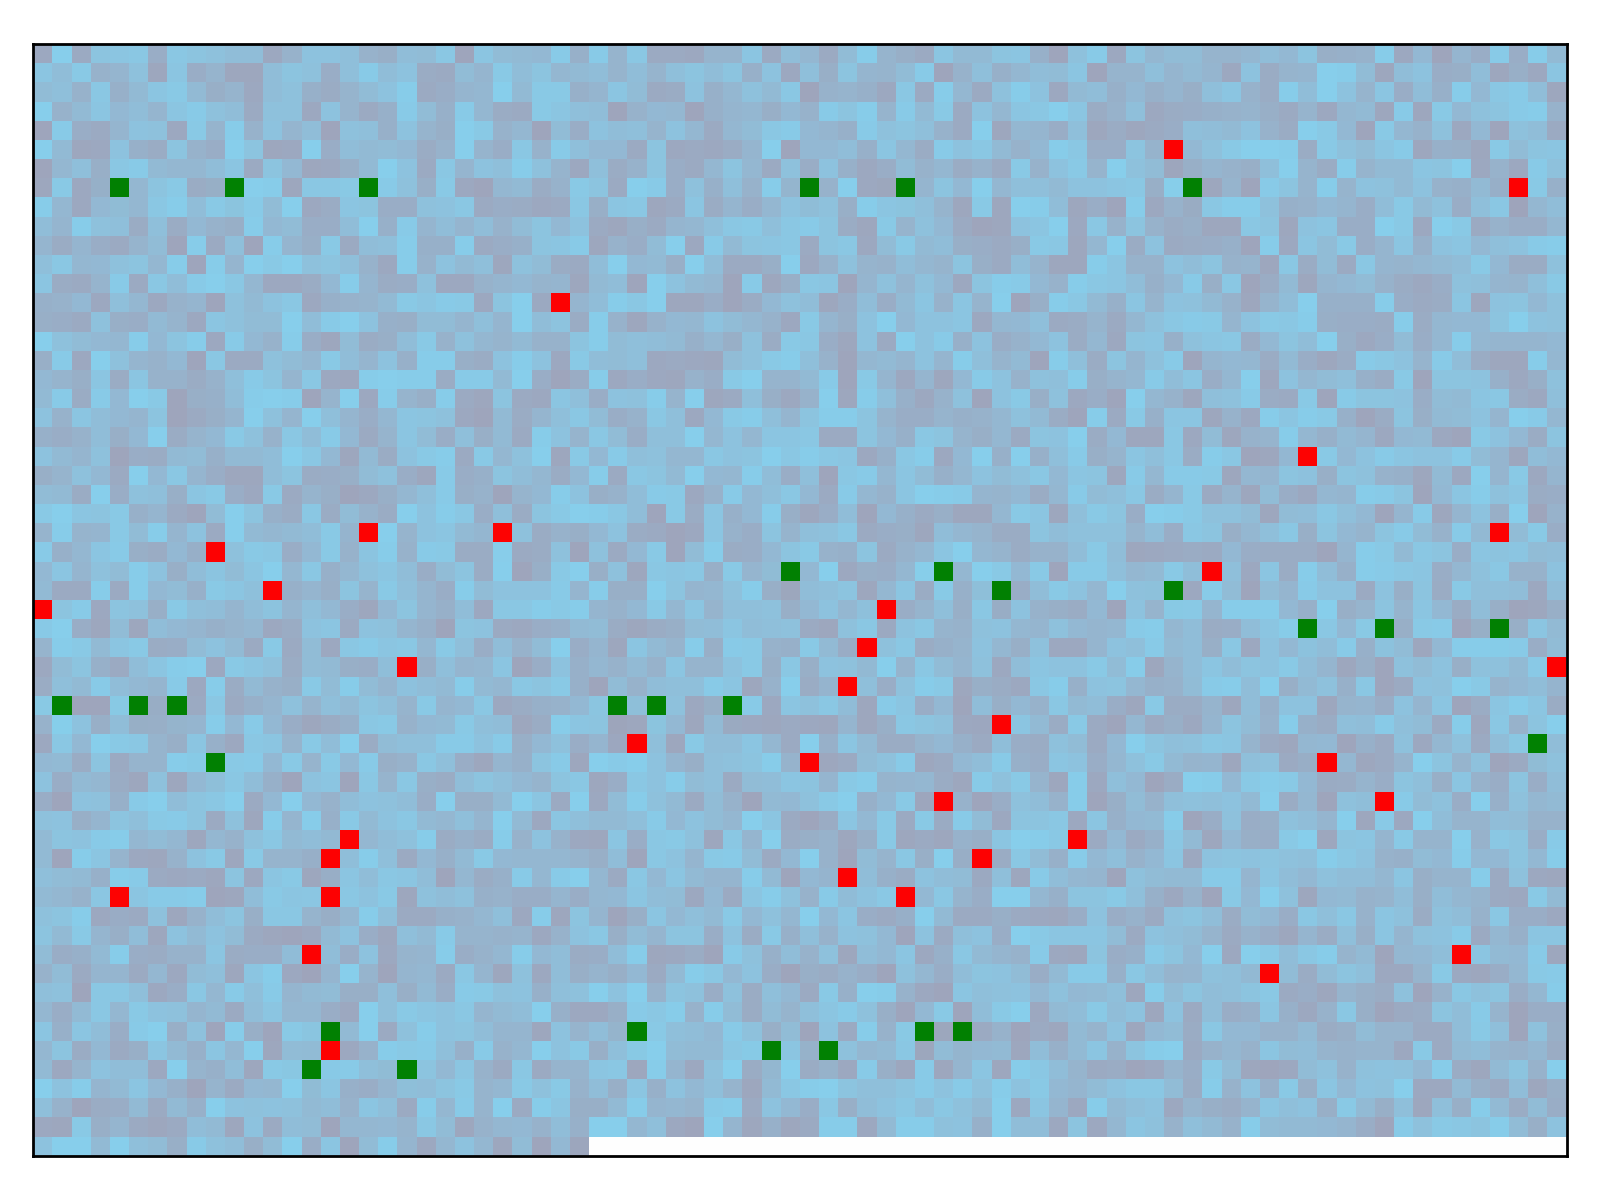
\includegraphics[width=0.75\textwidth]{doc11358_topic0.png} %&
        % 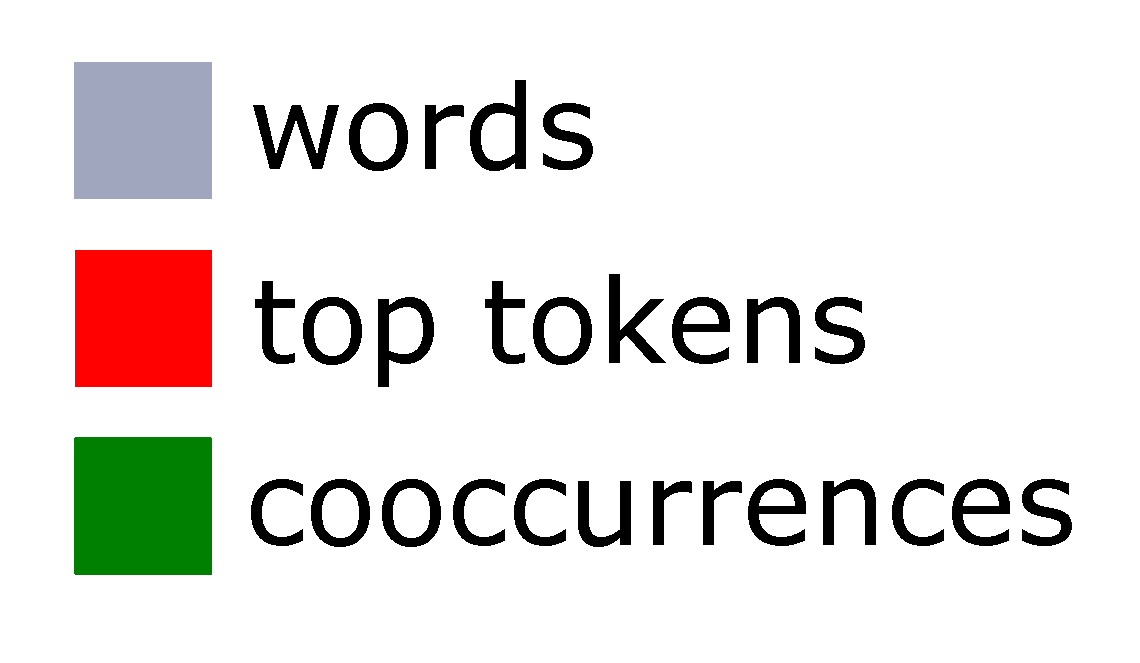
\includegraphics[width=0.25\textwidth]{legend.eps} \\
    %\end{tabular}
    \captionsetup{justification=raggedright,singlelinecheck=false,format=hang}
    \caption{Демонстрация доли текста, покрытой верхними словами, на примере одного документа. Словопозиции обозначены серо-синим цветом, словопозиции верхних слов показаны красным цветом, зелёным цветом показаны словопозиции, имеющие ненулевой вклад в расчёт когерентности (т.е. попадающие в скользящее окно вместе с другим верхним словом).}
\label{fig:ch3_doc_compound_auto}
\end{figure}

Также в этой главе предлагаются несколько мер качества, основанных на идее \textit{внутритекстовой когерентности}.
Традиционные меры когерентности сначала выделяют небольшое множество верхних слов в заданной теме по их $\phi_{wt}$ и затем анализируют, каким образом эти слова встречаются в тексте (анализ \emph{от темы к тексту}). В предлагаемом же методе сначала выделяются все соседние слова текста, распределение $\phi_{wt}$ которых затем анализируется (\emph{от текста к теме}).

Предполагается, что этот метод будет лучше характеризовать интерпретируемость тем, нежели традиционные меры когерентности. Эксперимент на полусинтетической коллекции показывает, что предлагаемый подход действительно отличается большей чувствительностью.

\underline{\textbf{В четвёртой главе}} рассматриваются способы увеличения интерпретируемости тематических моделей. Предложен метод подбора коэффициентов сглаживания, коэффициентов разреживания и весов дополнительных модальностей при помощи математического аппарата \textit{относительных коэффициентов}.

Эта техника облегчает построение тематических моделей, все темы которых различны и не <<загрязнены>> большим числом неинформативных токенов (слов общей лексики). Также она позволяет перенести имеющуюсся стратегию обучения тематической модели на другие текстовые коллекции схожей структуры.

Показано, что любому абсолютному коэффициенту сглаживания/разреживания $\Phi$ и $\Theta$ соответствует какой-то относительный коэффициент (и наоборот). Приводятся следующие формулы преобразований из $\lambda$ в $\tau$:

\begin{equation}
\tau = \frac{\lambda \sum_{d\in D} n_d }{(1-\lambda) |D| \cdot |T|} \label{sp_theta_rel2abs}
\end{equation}

\begin{equation}
\tau = \frac{n}{|T|\cdot|W|} \frac{\lambda}{(1-\lambda)}  \label{sp_phi_rel2abs}
\end{equation}

Регуляризатор сглаживания $\Theta$, воздействующий на темы $T$ и документы $D$, коэффициент $\tau$ которого вычислен по формуле \eqref{sp_theta_rel2abs}, можно проинтерпретировать как нахождение <<компромисса>>: результирующая $\Theta_{td}$ будет на $\lambda$ состоять из априорного распределения $\frac{1}{|T|}$ и на $(1-\lambda)$ из оценки максимума правдоподобия $\frac{n_{td}}{n_d}$.

Аналогично интерпретируется и формула \eqref{sp_phi_rel2abs} для регуляризатора сглаживания $\Phi$, воздействующего на темы $T$ и токены $W$. Здесь задаётся взвешенная комбинация из априорного распределения $\frac{1}{|W|}$ и оценки максимума правдоподобия $\frac{n_{wt}}{n_t}$.

Это означает, что любую существующую модель можно переформулировать в терминах относительного сглаживания и разреживания без каких-либо потерь. Практическая значимость этого результата заключается в вытекающей из него возможности переносить существующую схему сглаживания/разреживания на другую коллекцию схожей структуры.

Оставшаяся часть главы посвящена изучению роли матриц $\Phi$ и $\Theta$ в тематическом моделировании. Вопрос рассматривается с двух позиций: с точки зрения математической постановки задачи и с точки зрения построения и использования тематических моделей на практике. В терминах вероятностного смысла задачи обе матрицы являются равноправными.

При этом существует ряд причин, по которым естественно считать матрицу $\Theta$ второстепенной по отношению к $\Phi$. Особое значение для рассматриваемой работы имеет аргумент об интерпретируемости: описанный в предыдущей главе процесс оценки тем на интерпретируемость обычно состоит из выбора небольшого набора верхних слов для каждой темы и представления этого набора эксперту-человеку \cite{roder2015exploring}. В этом процессе используется только матрица $\Phi$. Таким образом, в контексте интерпретации найденных тем экспертами качество матрицы $\Phi$ оказывается более важным, чем качество матрицы $\Theta$.

В работе \cite{thetaless} доказывается, что введение функциональной зависимости $\Theta = f(\Phi)$ требует модификации EM-алгоритма. Эту модификацию можно истолковать, как добавление псевдорегуляризатора, что приводит к алгоритму быстрой векторизации документов на основании одной лишь матрицы $\Phi$. Именно в таком виде данный псевдорегуляризатор был интегрирован в открытую библиотеку TopicNet\footnote{\url{https://github.com/machine-intelligence-laboratory/TopicNet/blob/master/topicnet/demos/Topic-Thetaless-Regularizer.ipynb}}. 

Оставшаясся часть четвёртой главы посвящена изучению свойств этого псевдоргеуляризатора. Поведение модели с предложенным псевдоргеуляризатором исследуется на реальной текстовой коллекции. Результаты показывают, что этот псевдорегуляризатор действительно повышает ряд критериев качества, связанных с интерпретируемостью и успешно комбинируется с другими регуляризаторами.

\underline{\textbf{Пятая глава}} посвящена разработке библиотеке TopicNet. TopicNet --- открытая надстройка над библиотекой BigARTM, предоставляющая более удобные возможности для подбора гиперпараметров, для работы с пользовательскими регуляризаторами и для визуализации тематических моделей. Описанная библиотека доступна онлайн на GitHub.

Главная мотивация TopicNet --- создать инструмент, удобный как для новичков, так и для продвинутых пользователей. Большое внимание уделяется удобству работу и наличию <<рецептов моделирования>>, показывающих хорошее качество без трудоёмкой настройки гиперпараметров. Численный эксперимент показывает, что TopicNet с настройками <<по умолчанию>> превосходит модель LDA из открыто доступной библиотеки GenSim, также с настройками <<по умолчанию>>, по критериям различности, когерентности и информативности тем.

Библиотека TopicNet состоит из двух больших модулей: \texttt{Viewers} и \texttt{Cooking Machine}.  

Модуль \texttt{Viewers} содержит различные инструменты визуализации. Дизайн придерживается философии Unix: каждый вьювер имеет ограниченную область ответственности и способен возвращать результат операции в JSON-подобном виде.

Это даёт возможность комбинировать содержащиеся в модуле вьюверы, не теряя при этом удобные для конечного пользователя методы, возвращающие \texttt{pandas.DataFrame}, строку сформированного HTML, или отображающие результат сразу в ячейке вывода Jupyter Notebook. 

Модуль \texttt{Cooking Machine} содержит различные инструменты для моделирования, расположенные в иерархии основных классов. Эти классы отвечают за построение и обучение модели заданной структуры, за отбор моделей согласно заданным пользователем ограничениям, а также за сохранение, загрузку и журналирование происходящего процесса.

Процесс построения тематической модели представим в виде дерева. Каждый узел дерева содержит в себе тематическую модель, а ориентированные рёбра хранят информацию об отношениях <<предок-потомок>> вида <<модель $Y$ была получена из модели $X$ при помощи преобразования $T_{XY}$>>. Не все деревья эксперимента являются допустимыми. Мы накладываем ограничения на допустимые преобразования: требуем, чтобы все рёбра одного уровня описывали преобразования из одного и того же семейства, различающиеся лишь набором параметров. 

Одним из примеров таких преобразований является <<Применить к модели регуляризатор с произвольными параметрами>>. 

Класс \texttt{Experiment} отвечает за хранение, журналирование и актуализацию этой структуры.  

Все преобразования связаны с экземпляром класса \texttt{Cube}. Каждый \texttt{Cube} играет роль чертежа, задающего все преобразования на текущем уровне эксперимента. Таким образом, процесс обучения можно представить как цепочку кубов, последовательно соединённых друг с другом.  

Куб выполняет две важные функции. Первая --- это \textit{спецификация}: во время инициализации куб преобразует заданные пользователем параметры в многомерное пространство поиска. Вторая функция --- \textit{применение}: получив точку в пространстве поиска и тематическую модель, куб изменяет заданное множество параметров и/или гиперпараметров модели. Таким образом, он играет роль инкубатора для моделей, что отражено в названии класса. На Рис.  \ref{Training-scheme} приведена схема обучения, состоящая из двух кубов, применённых к одной модели.  

Классы \texttt{Experiment} и \texttt{Cube} позволяют сделать сложные стратегии обучения и журналирование экспериментов более сжатыми и доступными. Модуль \texttt{config\_parser} делает ещё один шаг в сторону облегчения конфигурируемости: стратегию обучения можно задать при помощи текстового конфигурационного файла в формате YAML.  

\begin{figure}[ht]
    \centering
    \captionsetup{justification=raggedright,singlelinecheck=false,format=hang}

    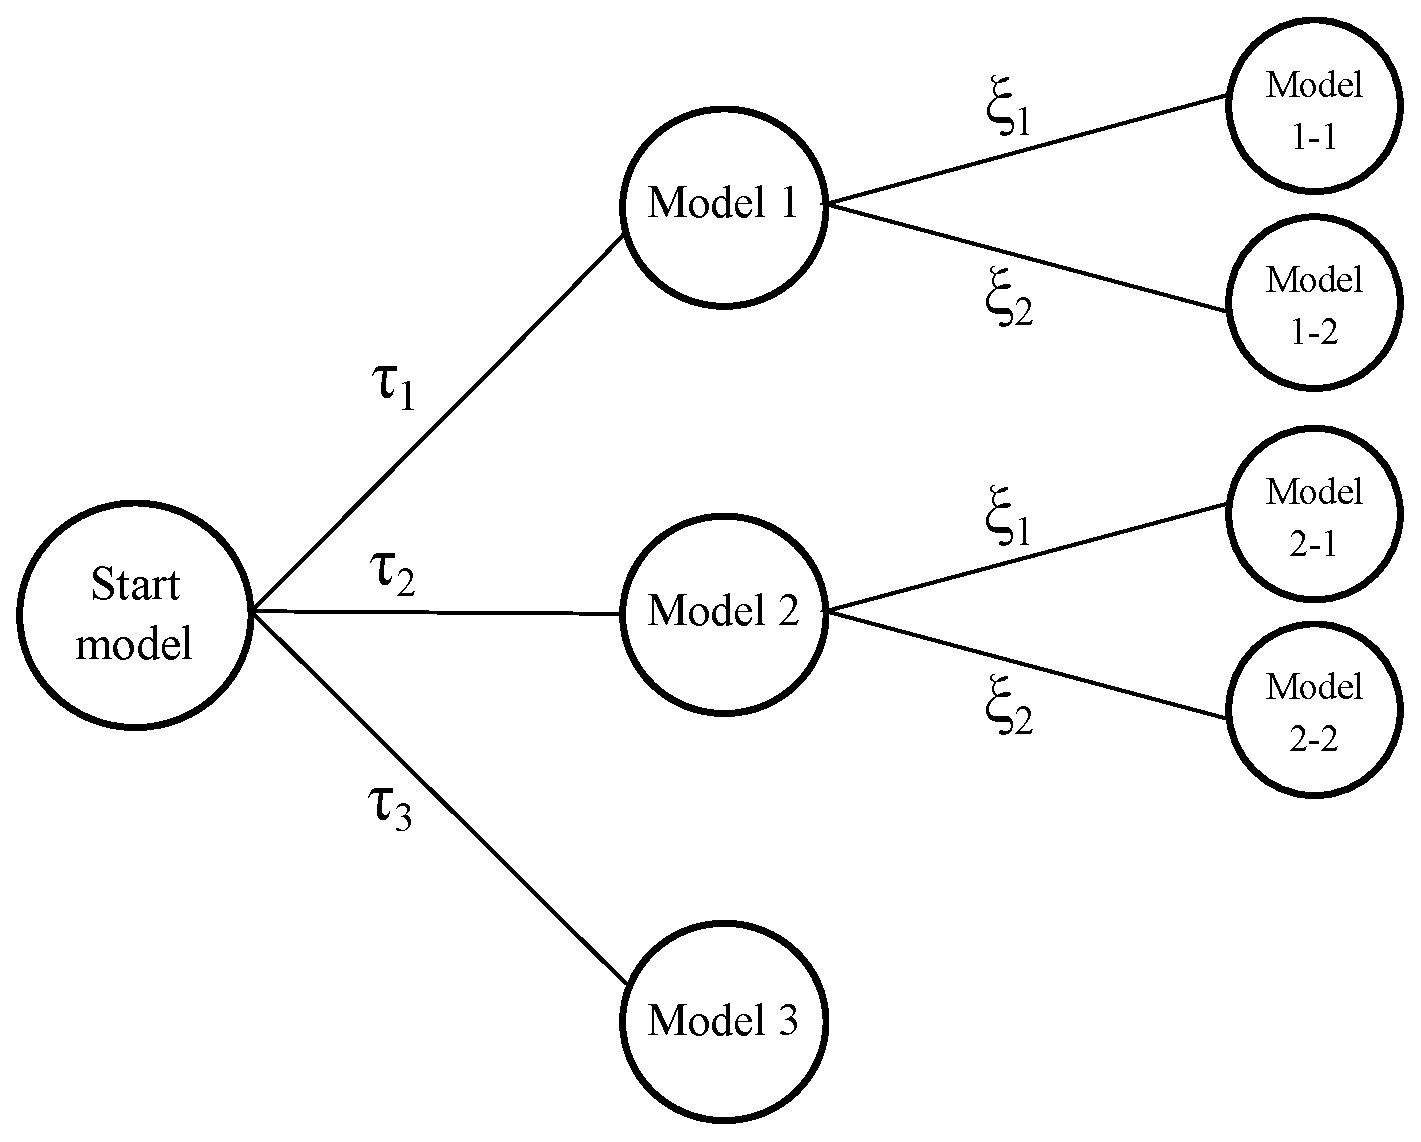
\includegraphics[width=0.7\textwidth]{training_scheme_example.eps}
    %\begin{flushleft}

    \caption{
        Пример двухэтапной схемы эксперимента.
        На первом этапе применяется регуляризатор с коэффициентом $\tau$, принимающим значения из некоторого множества $\{\tau_1, \tau_2, \tau_3\}$.
        Лучшими моделями после первого этапа являются \emph{Model 1} и \emph{Model 2}, поэтому \emph{Model 3} больше не участвует в процессе обучения.\\
        Второй этап связан с другим регуляризатором с коэффициентом $\xi$, принимающим значения из множества $\{\xi_1, \xi_2\}$.
        В результате этого этапа у каждой из ранее отобранных моделей  появляется два потомка.
    }
    %\end{flushleft}
\label{Training-scheme}
\end{figure} 


\begin{figure*}[ht]
% \footnotesize
\captionsetup{justification=raggedright,singlelinecheck=false,format=hang}
\texttt{TopicKernel@word.average\_contrast > 0.95 * MAXIMUM( \\
\hphantom{\ \ \ \ \ \ \ \ }TopicKernel@word.average\_contrast) \\
\hphantom{\ \ } and PerplexityScore@all < 1.1 * MINIMUM( \\
\hphantom{\ \ \ \ \ \ \ \ }PerplexityScore@all) \\
\hphantom{\ \ } and SparsityPhiScore@word -> max\\
\hphantom{\ \ } COLLECT 3} \\
\caption{Пример строки, задающей критерий отбора моделей. Здесь в качестве критериев отбора участвуют перплексия, контраст лексического ядра модальности \texttt{@word} и разреженность матрицы $\Phi$. Результатом будут три модели, контраст которых не более чем на 5\% отличается от наилучшего достигнутого контраста, имеют допустимую перплексию и как можно более разреженны. }
\label{DSL-example}
\end{figure*} 

В реальных экспериментах не у каждой модели есть потомки; большинство моделей отбрасывается в соответствии с каким-то критерием. Самый естественный, но в то же время самый трудозатратный способ анализа тематической модели --- это ручное изучение списков верхних токенов и верхних документов в темах, на основании которого пользователь принимает решение, какие из моделей являются <<удовлетворительными>>. Другой подход заключается в сравнении численных показателей; обычно используется перплексия и когерентность. Библиотека \mbox{BigARTM} добавляет к их числу дополнительные метрики разреженности, различности, чистоты и контрастности тем \cite{voron15mlj}, и другие.

Библиотека TopicNet также поддерживает пользовательские критерии качества. Значительная часть мер, описанных во второй главе, реализована на платформе TopicNet.  

Для того чтобы облегчить ручной анализ моделей, мы реализовали простой специализированный (domain-specific) язык для отбора моделей (пример приведён на Рис.~\ref{DSL-example}). Использование этого языка делает процесс многокритериального отбора моделей более простым и прозрачным.  

\underline{\textbf{В шестой главе}} рассматривается задача создания таксономии коллекции диалогов контактного центра без наличия разметки. Предлагается регуляризованная тематическая модель, играющая роль первого приближения к структуре коллекции.

Был использован усложнённый вариант распространённой техники, улучшающей интерпретируемость --- использования информативных $n$-грам (коллокаций) в качестве дополнительной модальности. Для того чтобы извлечь информативные $n$-грамы, был использован алгоритм TopMine~\cite{topmine}, основанный на статистике парной сочетаемости слов в текстовой коллекции.

Для нашей задачи имело смысл внести ряд правок в алгоритм TopMine. Во-первых, логика подсчёта статистик парной сочетаемости была модифицирована таким образом, чтобы в ней использовались мультимножества слов вместо последовательностей слов. 

Во-вторых, TopMine не выделяет пересекающиеся коллокации. Это приводит к тому, что похожие предложения (<<записать ребёнка в детский сад>> и <<записать ребёнка в детский садик>>) могут вовсе не содержать общих коллокаций. Примером служат предложение <<получение паспорта РФ>> (выделится коллокация \texttt{получение\_паспорт\_РФ}) и предложение <<паспорт РФ был утерян>> (выделится коллокация \texttt{паспорт\_РФ}). Это следует из процесса поиска коллокаций алгоритмом: на каждом шаге обработки соседние коллокации-кандидаты сливаются, если их объединение удовлетворяет критерию информативности. Для того чтобы устранить вышеописанную проблему, достаточно изменить процесс итеративного слияния фраз так, чтобы при успешном слиянии коллокаций они не удалялись из множества кандидатов. Данная модификация увеличивает потребление памяти алгоритмом, однако делает процесс поиска менее <<жадным>>.

% Во-первых, исходный алгоритм вычисляет статистики совстречаемости для упорядоченных кортежей слов $(w_1, w_2, \dots, w_k)$. В частности, алгоритм различает последовательности $(w_1, w_2)$ и $(w_2, w_1)$. Эта особенность делает алгоритм TopMine плохо приспособленными для обработки текстов на языках с нестрогим порядком слов (таких как русский). По этой причине логика подсчёта статистик совстречаемостей алгоритма была модифицирована таким образом, чтобы в ней использовались мультимножества слов вместо последовательностей слов.

Предлагаемая модель является двухуровневой, то есть состоит из двух <<обычных>> тематических моделей. Модель первого уровня и модель второго ориентируются на различные признаки. Это связано с тем, что первый уровень иерархии предназначен для определения предмета диалога, а цель второго уровня иерархии --- нахождение действий, о которых говорит пользователь. % Существительные имеют большое влияние на темы первого уровня, а для тем второго уровня более важную роль играют глаголы.

В контексте поставленной задачи было предпринято разделение признаков по их функциональному назначению. Из всех токенов (слов и $n$-грам) были выделены две группы на основании их частеречного состава: <<тематическая>> и <<функциональная>>. <<Функциональная>> группа состоит из одиночных глаголов и $n$-грам, содержащих хотя бы один глагол. <<Тематическая>> группа состоит из одиночных существительных, одиночных прилагательных и $n$-грамм, включающих в себя хотя бы одно существительное и не имеющих в своём составе глаголов.

Таким образом, предлагаемая тематическая модель использует пять модальностей: \texttt{@lemmatized} (просто слова), \texttt{@verb\_lemmatized} (слова-глаголы), \texttt{@noun\_lemmatized} (слова-существительные и слова-прилагательные), \texttt{@theme\_ngramms} ($n$-грамы с существительными и без глаголов), \texttt{@verb\_ngramms} ($n$-грамы с глаголами).

Одна и та же стратегия обучения успешно применяется к двум разным коллекциям диалогов. Первая коллекция состоит из диалогов клиентов с представителями различными государственных организаций, а вторая представляет собой логи технической поддержки провайдера. Механизм относительных коэффициентов позволил успешно перенести веса модальностей, подобранные на первой коллекции, на вторую коллекцию.

\FloatBarrier
\pdfbookmark{Заключение}{conclusion}                                  % Закладка pdf
В \underline{\textbf{заключении}} приведены основные результаты работы, которые заключаются в следующем:
%% Согласно ГОСТ Р 7.0.11-2011:
%% 5.3.3 В заключении диссертации излагают итоги выполненного исследования, рекомендации, перспективы дальнейшей разработки темы.
%% 9.2.3 В заключении автореферата диссертации излагают итоги данного исследования, рекомендации и перспективы дальнейшей разработки темы.
\begin{enumerate}[beginpenalty=10000]
\item
    Методология построения аддитивно регуляризованных тематических моделей, обеспечивающая формирование <<рецептов моделирования>> с автоматизированным подбором гиперпараметров по множеству критериев и отличающаяся использованием относительных коэффициентов регуляризации и кубов гиперпараметров.
\item
    Архитектура библиотеки TopicNet, обеспечивающая программную реализацию данной методологии и отличающаяся использованием удобного языка описания кубов гиперпараметров и возможностью создания пользовательских регуляризаторов и метрик качества на языке Python.
\item
    Универсальный рецепт моделирования, обеспечивающий многокритериальный выбор тематических моделей для широкого класса задач, отличающийся предварительной настройкой куба гиперпараметров по набору разнородных задач тематического моделирования.
\item
    Программная реализация нового критерия когерентности, обеспечивающая его эффективное вычисление и отличающаяся более полным использованием данных о сочетаемости слов внутри текстовых документов.
%\item
%    Программная реализация псевдорегуляризатора в библиотеке TopicNet, обеспечивающего быстрое однопроходное вычисление тематических векторных представлений документов и улучшение качества тематической модели по множеству критериев.
\end{enumerate}




\pdfbookmark{Литература}{bibliography}                                % Закладка pdf

% При использовании пакета \verb!biblatex! список публикаций автора по теме диссертации формируется в разделе <<\publications>>\ файла \verb!common/characteristic.tex!  при помощи команды \verb!\nocite!

\ifdefmacro{\microtypesetup}{\microtypesetup{protrusion=false}}{} % не рекомендуется применять пакет микротипографики к автоматически генерируемому списку литературы
\urlstyle{rm}                               % ссылки URL обычным шрифтом
\ifnumequal{\value{bibliosel}}{0}{% Встроенная реализация с загрузкой файла через движок bibtex8
  \renewcommand{\bibname}{\large \bibtitleauthor}
  \nocite{*}
  \insertbiblioauthor           % Подключаем Bib-базы
  %\insertbiblioexternal   % !!! bibtex не умеет работать с несколькими библиографиями !!!
}{% Реализация пакетом biblatex через движок biber
  % Цитирования.
  %  * Порядок перечисления определяет порядок в библиографии (только внутри подраздела, если `\insertbiblioauthorgrouped`).
  %  * Если не соблюдать порядок "как для \printbibliography", нумерация в `\insertbiblioauthor` будет кривой.
  %  * Если цитировать каждый источник отдельной командой --- найти некоторые ошибки будет проще.
  %
  \nocite{intracoh, popov_hier, bulatov2020topicnet, thetaless}

  %% authorprogram
  \nocite{prog_cook}%
  \nocite{prog_stkc}%
  \nocite{prog_view}%
  %

  \ifnumgreater{\value{usefootcite}}{0}{
    \begin{refcontext}[labelprefix={}]
      \ifnum \value{bibgrouped}>0
        \insertbiblioauthorgrouped    % Вывод всех работ автора, сгруппированных по источникам
      \else
        \insertbiblioauthor      % Вывод всех работ автора
      \fi
    \end{refcontext}
  }{
  \ifnum \totvalue{citeexternal}>0
    \begin{refcontext}[labelprefix=A]
      \ifnum \value{bibgrouped}>0
        \insertbiblioauthorgrouped    % Вывод всех работ автора, сгруппированных по источникам
      \else
        \insertbiblioauthor      % Вывод всех работ автора
      \fi
    \end{refcontext}
  \else
    \ifnum \value{bibgrouped}>0
      \insertbiblioauthorgrouped    % Вывод всех работ автора, сгруппированных по источникам
    \else
      \insertbiblioauthor      % Вывод всех работ автора
    \fi
  \fi
  %  \insertbiblioauthorimportant  % Вывод наиболее значимых работ автора (определяется в файле characteristic во второй section)
  \begin{refcontext}[labelprefix={}]
      \insertbiblioexternal            % Вывод списка литературы, на которую ссылались в тексте автореферата
  \end{refcontext}
  
  % Невидимый библиографический список для подсчёта количества внешних публикаций
  % Используется, чтобы убрать приставку "А" у работ автора, если в автореферате нет
  % цитирований внешних источников.
  % \printbibliography[heading=nobibheading, section=1, keyword=biblioexternal]%
  }
}
\ifdefmacro{\microtypesetup}{\microtypesetup{protrusion=true}}{}
\urlstyle{tt}                               % возвращаем установки шрифта ссылок URL
      % Содержание автореферата

\iffalse
%%% Выходные сведения типографии
\newpage\thispagestyle{empty}

\vspace*{0pt plus1fill}

\small
\begin{center}
    \textit{\thesisAuthor}
    \par\medskip

    \thesisTitle
    \par\medskip

    Автореф. дис. на соискание ученой степени \thesisDegreeShort
    \par\bigskip

    Подписано в печать \blank[\widthof{999}].\blank[\widthof{999}].\blank[\widthof{99999}].
    Заказ № \blank[\widthof{999999999999}]

    Формат 60\(\times\)90/16. Усл. печ. л. 1. Тираж 100 экз.
    %Это не совсем формат А5, но наиболее близкий, подробнее: http://ru.wikipedia.org/w/index.php?oldid=78976454

    Типография \blank[0.5\linewidth]
\end{center}
\cleardoublepage
\fi
\end{document}
